%%%%%%%%%%%%%%%%%%%%%%%%%%%%%%%%%%%%%%%%%%%%%%%%%%%%%%%%%%%%%%%%%%%%%%%%
%                                                                      %
% LaTeX, FIIW thesis template                                          %
% 19/12/2023 v1.3                                                      %
%%%%%%%%%%%%%%%%%%%%%%%%%%%%%%%%%%%%%%%%%%%%%%%%%%%%%%%%%%%%%%%%%%%%%%%%
\documentclass[11pt,a4paper]{report}
% If you want to print a recto-verso version, use the documentclass below
%\documentclass[11pt,a4paper,twoside,openright]{report}


%%%%%%%%%%%%%%%%%%%%%%%%%%%%%%%%%%%%%%%%%%%%%%%%%%%%%%%%%%%%%%%%%%%%%%%%%%%%%%%%%%%%%%%%%%%%%%%%%%%%
% LaTeX packages                                                                                   %
%%%%%%%%%%%%%%%%%%%%%%%%%%%%%%%%%%%%%%%%%%%%%%%%%%%%%%%%%%%%%%%%%%%%%%%%%%%%%%%%%%%%%%%%%%%%%%%%%%%%

% 页边距设置
\usepackage[a4paper,left=2.5cm, right=2.5cm, top=3.5cm, bottom=3.5cm]{geometry}

% 语言与输入
\usepackage[utf8]{inputenc}         % UTF-8 编码
%\usepackage{babel}                  % 多语言支持(根据需要添加)

% 图像
\usepackage{graphicx}
\graphicspath{{./figs/}}

% 数学相关
\usepackage{amsmath}
\usepackage{amssymb}
\usepackage{mathtools}
\usepackage{siunitx}
\sisetup{detect-all}

% 表格相关
\usepackage{array}
\usepackage{booktabs}
\usepackage{multirow}
\usepackage{tabularx}
\usepackage{longtable}

% 代码高亮与显示
\usepackage{listings}
\lstset{
    breaklines=true,        
    breakatwhitespace=true, 
    basicstyle=\ttfamily\small, 
    columns=fullflexible
}
\usepackage{verbatim}
\usepackage{minted}
\usemintedstyle{borland}

% 算法环境
\usepackage{algorithm}
\usepackage{algorithmicx}
\usepackage{algpseudocode}

% 超链接与网址
\usepackage{hyperref}
\usepackage{url}
\hypersetup{
    colorlinks=true,
    breaklinks=true,
    urlcolor=blue,
    linkcolor=black,
    citecolor=black
}
\def\UrlBreaks{\do\/\do-}
\urlstyle{same}

% PDF 插入
\usepackage[final]{pdfpages}

% 图片子图
\usepackage{subfig}
\usepackage{float} % 提供 H 选项

% 图注
\usepackage[labelfont=bf]{caption}

% biblatex: citations from 'references.bib'
\usepackage[backend=biber, style=ieee, citestyle=numeric-comp, maxnames=99]{biblatex}
\addbibresource{references.bib}
\AtBeginBibliography{\footnotesize}
% 符号与缩略语表
\usepackage[acronym,toc]{glossaries}
\renewcommand{\glossarysection}[2][]{} % 禁用 glossary 标题


% 符号表样式
\newglossary*{symbols}{}
\glsaddkey{unit}{\glsentrytext{\glslabel}}{\glsentryunit}{\GLsentryunit}{\glsunit}{\Glsunit}{\GLSunit}
\newglossarystyle{symbolsStyle}{%
    \setglossarystyle{long3col}
    \renewenvironment{theglossary}{%
        \renewcommand*{\arraystretch}{1}%
        \begin{longtable}{p{0.1\textwidth}p{0.8\textwidth}>{\centering\arraybackslash}p{0.1\textwidth}}%
    }{%
        \end{longtable}%
    }
    \renewcommand*{\glossaryheader}{\endhead}
    \renewcommand*{\glossentry}[2]{%
        \glstarget{##1}{\glossentryname{##1}}%
        & \glossentrydesc{##1}%
        & [\glsunit{##1}] \tabularnewline
    }
}
\newglossarystyle{acronymsStyle}{%
    \setglossarystyle{long3col}
    \renewenvironment{theglossary}{%
        \renewcommand*{\arraystretch}{0.5}%
        \begin{longtable}{p{0.1\textwidth}p{0.9\textwidth}>{\centering\arraybackslash}p{0\textwidth}}%
    }{%
        \end{longtable}%
    }
    \renewcommand*{\glossaryheader}{\endhead}
    \renewcommand*{\glossentry}[2]{%
        \glstarget{##1}{\glossentryname{##1}}%
        & \glossentrydesc{##1}%
        & \tabularnewline
    }
}
\makeglossaries
% TikZ 绘图
\usepackage{tikz}
\usetikzlibrary{positioning, arrows.meta}

% mhchem: Chemical formulas (e.g.: \ce{CO2})
\usepackage[version=4]{mhchem}

% longtable, tabularx, booktabs, array: for improved tables
\usepackage{longtable}
\usepackage{tabularx}
\usepackage{booktabs}
\usepackage{array}

% packages to match word template fonts as closely as possible
\usepackage{helvet}
\renewcommand{\familydefault}{\sfdefault}
\usepackage{courier}

%%%%%%%%%%%%%%%%%%%%%%%%%%%%%%%%%%%%%%%%%%%%%%%%%%%%%%%%%%%%%%%%%%%%%%%%%%%%%%%%%%%%%%%%%%%%%%%%%%%%
% FIIW template setup                                                                              %
%%%%%%%%%%%%%%%%%%%%%%%%%%%%%%%%%%%%%%%%%%%%%%%%%%%%%%%%%%%%%%%%%%%%%%%%%%%%%%%%%%%%%%%%%%%%%%%%%%%%
% NOTE: doclang only sets the language of document titles AFTER the title/copyright pages
\def\doclang{english} % Eng: use 'english'
\usepackage{fiiw}
%\usepackage{natbib}						% used for cites from the bib file in your text
\usepackage{listings}             		% used for displaying source code (java, c, matlab,...)
\usepackage{verbatim}					% used for inline formatting of source code, terminal commands, 
\usepackage{hyperref}					% include hyperlinks in the resulting PDF
\usepackage{url}						% add url's with \url{http://}
\usepackage{subfig}
\usepackage{amsmath}					% extend math features
\usepackage[final]{pdfpages}            % include pdf's e.g.: a paper or a poster
\usepackage{float}                      % adds [H] to figure env. Puts a figure where you want it e.g. \begin{figure}[H]
\usepackage{longtable}					% used for tables that strech over muliple pages

%\usepackage[toc, acronyms]{glossaries}	% used by the list of symbols

% voorwoord (Eng: preface)
\acknowledgementspagetrue
\acknowledgements{voorwoord} % uses 'voorwoord.tex' for the preface
% abstract
\abstractpagetrue
\abstract{abstract.tex}
% dutch abstract (samenvatting)
\abstractnlpagetrue
\abstractnl{samenvatting.tex}
% lijst van figuren (Eng: list of figures)
\listoffigurespagetrue
% lijst van tabellen (Eng: list of tables)
\listoftablespagetrue
% lijst van symbolen (Eng: list of symbols)
%\listofsymbolspagetrue
%\listofsymbols{symbolen.tex}
% lijst van afkortingen (Eng: list of abbreviations)
\listofacronymspagetrue
\listofacronyms{afkortingen.tex}

% education, specialisation
\opleiding{Elektronica-ICT} % Eng: Electronics-ICT
% campuses: denayer, geel, gent, groept, brugge (denayereng, geeleng, ghenteng, groupteng, brugeseng)
\campus{groupteng}
%\embargo{01-01-1970}

% thesis title, author, promotor(s), etc.
\title{Neural Network Compression for Vision Applications in Space}
\subtitle{}
\academicyear{2024 - 2025}
\forenameA{Zhengchi}
\surnameA{Wu}
% leave second author (B) open if unused
\forenameB{}
\surnameB{}
% Eng: Supervisor(s), Co-supervisor(s)
\promotorA[Promotor]{\mbox{Prof. Dr Ing Peter Karsmakers}}
\promotorB[Co-promotor]{Ing Toon Vinck\anotherPromotor %Mijn 2e co-promotor\anotherPromotor Mijn bedrijfspromotor
} % co-promotor, company promotor, etc. names


%%%%%%%%%%%%%%%%%%%%%%%%%%%%%%%%%%%%%%%%%%%%%%%%%%%%%%%%%%%%%%%%%%%%%%%%%%%%%%%%%%%%%%%%%%%%%%%%%%%%
% Actual LaTeX document                                                                            %
%%%%%%%%%%%%%%%%%%%%%%%%%%%%%%%%%%%%%%%%%%%%%%%%%%%%%%%%%%%%%%%%%%%%%%%%%%%%%%%%%%%%%%%%%%%%%%%%%%%%
\begin{document}
\selectlanguage{\doclang}
\preface%
\clearpage

\chapter{Introduction}

Over the past years, deep learning technology has rapidly advanced to normalize using \gls{dnn} as one of the key techniques in the area of computer vision. DNNs have achieved state-of-the-art performance, outperforming previous traditional techniques and even humans, on tasks like image classification \cite{deng2009imagenet}, object detection \cite{redmon2016you}, image segmentation \cite{ronneberger2015u}, and behavior recognition \cite{carreira2017quo}. AI has made a paradigm shift in terms of "perception" to "cognition" predominantly aided by recent advances in computer vision through \gls{cnn} and attention-based architectures(e.g., Transformer).

As the scope of space activities has expanded, the necessity of developing methodologies to transfer visual intelligence capabilities to a range of space platforms has emerged as a new area of research interest. This includes orbital spacecraft, interstellar probes, and deep space exploration vehicles. Future space missions, especially highly automated missions such as orbital debris identification, autonomous navigation and obstacle avoidance, unknown terrain identification and surveying, and astronaut assistance operations will be entirely dependent on the capabilities of computer vision systems for real-time processing and real-time judgment \cite{Zhang2022}. 



Indeed, several actual or planned space missions have incorporated visual recognition modules into their core subsystems, which is an early stage in the exploration of deploying space AI systems. Examples include:

\begin{itemize}

  \item \textbf{The NASA Perseverance Mars Rover}: equipped with multiple cameras and computer vision systems for mapping the Martian surface, identifying rocks, steering and avoiding obstacles, etc. Its autonomous navigation system processes ground information through visual recognition to achieve path planning, markedly decreasing the frequency of ground intervention. \cite{NASAPerseverance}

   

  \item \textbf{The ESA Hera asteroid mission}: planned to travel to the Didymos binary asteroid system, the mission relies on a visual module to recognize asteroid surface morphology and perform 3D modeling, providing a key reference for future planetary defense technology. \cite{ESAHera}

   

  \item \textbf{NASA OSIRIS-REx asteroid mission}: During the approach to the asteroid Bennu, image recognition was used to select a suitable sampling area, and the trajectory was adjusted in real-time to achieve precision guidance. This is a typical example of early visual navigation used for sampling control. \cite{Lauretta2017}

   

  \item The Chinese Tianwen-1 Mars exploration mission: Visual navigation and terrain recognition systems are widely used during the landing and patrol phases of Mars to assist with landing site selection and path planning, demonstrating highly integrated visual reasoning capabilities. \cite{Tianwen1}

   

  \item NASA's Artemis lunar mission and Lunar Gateway: Computer vision systems are planned to be deployed for object detection inside/outside the mission module, robot collaboration, and system maintenance assistance, which are key components of intelligent vision in deep space manned missions. \cite{NASAArtemis}

\end{itemize}



According to the European Space Agency \cite{ESAHera}and the US National Aeronautics and Space Administration (NASA) in their white paper “Artificial Intelligence for Space Missions”, “The local reasoning capabilities of the AI systems in space will be key to enabling a revolution in the evolution of space missions from automation to intelligence.” \cite{NASA_AI_Space} . 



Nonetheless, deploying highly advanced DNN models in space missions are subject to many limitations. First, DNN models tend to be large and computationally expensive. As an example, ResNet-50 is a classic deep \gls{cnn} which was designed with a residual connection mechanism to effectively alleviate or mitigate the problem of gradient vanishing in deep networks \cite{glorot2010understanding}. This particular network possesses 50 hierarchical structures that include convolutional layers, batch normalization layers, activation functions, and residual blocks. With regard to these 50 structures, ResNet-50 has approximately 25.6 million parameters, and it requires about 4.1 billion \gls{flops} per inference \cite{he2016deep}. ResNet-50 is extensively used for many image classification and detection tasks and demonstrates remarkable efficacy on the ImageNet dataset.



Another sophisticated architecture is the self-attention-based \textbf{\gls{vit}} \cite{dosovitskiy2020image}. In contrast to the conventional image recognition models based on \gls{cnn}, \gls{vit} splits an image into equal-sized patches (or tokens) and then treats them as a sequence input into the Transformer encoder. As with the popular \textbf{\gls{vit}-Base} model mentioned earlier, there are 12 Transformer encoder layers, and each layer has 12 attention heads, allowing the model parameters to reach numbers upwards of \textbf{86 million}. Each inference requires roughly about \textbf{17.6 billion \gls{flops}} per the model’s architecture, presenting a substantially higher requirement for memory bandwidth and computing resources than the ResNet series. Despite this high computational overhead, the architectures are successfully run on terrestrial platforms with the use of accelerator devices that provide good performance, such as the NVIDIA V100, A100 GPU, or Apple M series chip; however, when deploying onto space platforms, the architectures face severe real-world constraints. Space vehicle processors require robust radiation tolerance and high reliability, often sacrificing performance in return. Many of the current generation mainstream radiation tolerant processors installed on the space vehicle include



\begin{itemize}

  \item \textbf{RAD750} (BAE Systems): based on the PowerPC 750 architecture, with a clock speed of only 133~MHz, 128~MB~SDRAM, and peak computing performance of about \textbf{266 \gls{mips}}, widely used in NASA missions such as Curiosity and Perseverance \cite{rad750};

  \item \textbf{LEON3/LEON4} (Cobham Gaisler): based on the SPARC architecture, operating frequency about 100-250~MHz, peak performance of hundreds of~MIPS, used in several ESA deep space missions \cite{leon34};

  \item \textbf{GR740}: a quad-core LEON4FT chip developed by the European Space Agency, with a clock speed of 250~MHz, support for 1~GB DDR3, and a peak performance of about 1~GFLOPs \cite{gr740}.

\end{itemize}



In contrast, AI accelerators used on the ground have computing power that is thousands of times greater. As shown in Table~\ref{tab:gpu_comparison}, the NVIDIA V100, NVIDIA A100, and Apple M1/M2 series have distinctive performance characteristics.

\begin{table}[H]
  \centering
  \caption{Comparison between Ground-based GPUs and Space Processors}
  \label{tab:gpu_comparison}
  \renewcommand{\arraystretch}{1.2}  % 调整行距
  \setlength{\tabcolsep}{4pt}        % 调整列间距
  \begin{tabularx}{1\textwidth}{%
      >{\raggedright\arraybackslash}p{2.5cm}  % Processor
      >{\raggedright\arraybackslash}p{1.5cm}  % Platform
      >{\raggedright\arraybackslash}X          % Key Specifications
  }
    \toprule
    \textbf{Processor} & \textbf{Platform} & \textbf{Key Specifications} \\
    \midrule
    GR740 
      & Space 
      & Quad-core LEON4FT, 250~MHz clock, 1~GB DDR3, peak performance of ~1~GFLOPS. \\
    \midrule
    NVIDIA V100 
      & Ground 
      & Volta architecture, 5,120 CUDA cores, 4,096 Tensor cores, 15.7~TFLOPS (FP32), 32~GB HBM2. \\
    \midrule
    NVIDIA A100 
      & Ground 
      & Ampere architecture, up to 19.5~TFLOPS (FP16) or 312~TFLOPS (Tensor Core BF16), supports 40~GB/80~GB HBM2e. \\
    \midrule
    Apple M1/M2 Series 
      & Ground 
      & Integrated Neural Engine, e.g., the M2 Neural Engine executes up to 15.8 billion operations per second (TOPS). \\
    \bottomrule
  \end{tabularx}
\end{table}






In comparing magnitude, the most powerful space processors currently define computing just above 1 GFLOPS, such as the GR740, whereas GPUs on the ground can easily achieve between 10 and 100+ TFLOPS. This means the millions of operations required by traditional ground-based deep learning models during the inference will still be executed over a period of anywhere between tens and hundreds of seconds on the space processor, and no longer adequate for real-time processing on these platforms. Furthermore, there are substantial, specific limitations of space platforms in terms of power, heat dissipation, reliability, and storage bandwidth, which drive the need for lightweight, low-power, and robust deep learning models. 



More importantly, the radiation conditions in space will create a series of reliability risks. Solar storms, galactic cosmic rays, and high-energy particle streams will constantly bombard electronic systems, creating issues such as \gls{seu} and \gls{sel}. For \gls{dnn}, these upsets can affect the weight parameters, values for input activations, or even to the connections between the neurons, making errors on inference the same experience without alarm for the hardware level failure detection.



Experiments and simulations in realistic radiation environments suggest that the chance of a bit‐flip occurring in a floating point weight of 16 bits is about 1 in 10,000 per hour. \cite{venables2003enhancing}


Accordingly, to the point that, a model with tens of millions of parameters can accrue several random damages in a matter of hours; and since \gls{dnn} models are highly nonlinear and can amplification minor perturbations, this “silent data corruption” can potentially result serious misalignment in the inference stage. An example would be in the way the \gls{dnn} would associate orbital debris with "Orbital gravel" haul, instead of "mission equipment" which would impact the robotic arm underpinning the orbital grasping or orbital avoidance planning with the end user resulting in a catastrophic mission failure.



To address the above challenges, academia and industry have proposed many optimization methods to reduce the operational complexity and sensitivity of \gls{dnn} models. For example:

\begin{itemize}

  \item \textbf{Model quantization (Quantization)}:Compress 32-bit floating-point representations to 8-bit or even 4-bit integers significantly reduces model storage and multiply-add operation costs \cite{howard2017mobilenet}. Studies have shown that 8-bit \gls{ptq} can reduce the amount of computation by about 4 times without significantly affecting accuracy.

  \item \textbf{Pruning}: Sparsity the model by pruning redundant neurons, convolutional kernels, or attention heads, thereby reducing the complexity of the computational graph \cite{raina2009large}.

  \item \textbf{Knowledge Distillation}: Training a small model to imitate the output of a large model to improve the performance of a compact model.

  \item \textbf{Neural Architecture Search}: uses a search algorithm to find the network structure that performs best on a particular piece of hardware.

\end{itemize}



Although these methods are widely used on mobile devices and edge AI devices (such as smartphones and embedded terminals), most of them ignore the impact of the radiation environment on the model \cite{Souvatzoglou2024}.
Modern models of \gls{dnn} often show an upper bound on tradeoff between model size or number of \gls{flops} and robustness to fault. The motivation for this study is that larger \gls{dnn} are naturally more redundant and could potentially be more robust to soft errors such as \gls{seu} compared with smaller, pruned models. In constrained situations, like space, where computational limits and radiation-induced errors are performance barriers, understanding the trade-off will help familiarize engineers with the underlying mechanisms and strategies that can be adopted.
The primary research question for this study is as follows: To what extent does model pruning impact the robustness of neural networks against \gls{seu}? The current study will specifically analyze how structured pruned models that impact \gls{flops} impacts classification accuracy under deterministic fault injection. The objective of the current study is to assess whether lightweight but high-capacity networks can be robust enough to be deployed for fault tolerant, application-specific uses in space-borne vision systems.



In summary, this study integrates three key techniques: quantitative analysis, structured pruning, and dynamic reconstruction. By simulating errors generated in the model under high-radiation conditions in the universe, it clarifies the relationship between the model's \gls{flops} and accuracy after error injection. This research not only fills a critical gap in the field of reliability for space artificial intelligence models but also provides essential technical support for high-risk tasks such as deep space exploration, lunar base construction, and autonomous orbital visual navigation.

The rest of the remaining chapters structured as follows: Chapter \ref{chap:design} defines some on the principles of constructing and training neural networks, in addition to regularization (dropout) techniques and to explain the reasoning behind structured pruning to test spacecraft constraints. Chapter \ref{chap:imp} contains the structured pruning, quantization, and dynamic reconstruction, on both the VGG and CCDF\_MNIST models and establishes a methodical model error injection. Chapter \ref{chap:evaluation} provides experimental results and analysis between different pruning levels (\gls{flops} reduction) with classification accuracy on bit-flipping injection, and their relevant fault-tolerance curves. Chapter \ref{chap:discussion} discusses the relationship of the research results to the existing work and highlights the weaknesses. Finally, chapter \ref{chap:conclusion} summarizes the key contributions of this research, brings together the research results, and describes potential directions for future work.
\chapter{Design and Materials}
\label{chap:design}
\section{Introduction of this chapter}
An \gls{ann}, is a computational model based on the idea that the brain is comprised of interconnected neurons of varying types and connectivity. \gls{ann} also consist of many simple processing elements or "neurons," and can have one or more layers of neurons. Typically, each neuron will have many inputs, they will process the inputs by weighing and summing the input to produce an output (plus one bias), and then a nonlinear activation function is used to produce the last output of the particular neuron. By connecting many layers of these neurons, \gls{ann} can be trained to map complex, nonlinear functions to outputs from raw inputs (pixel intensities or sensor readings) to outputs (class labels or continuous predictions). In this chapter we will set out the basic underpinnings for building , training a neural network, describe why we bother building neural networks and how is it related to our research objective





\section{Introduction to Neural Networks} 
Neural networks now underpin most current state-of-the-art artificial intelligence, in part because of their plausible similarity to human brain information processing. We will identify the basic features of neural networks, and introduce some very rough analogies to help conceptualize the new structures while maintaining appropriate mathematical development. This does indicate a solution that intertwines biology and mathematics that is also flexible and adaptable to convoluted problems in the real world.











\section{Inspiration of Neural Networks}

The first mathematical representation of a neuron was presented by McCulloch and Pitts, who abstracted biological neurons to simplistic binary logic functions. This conceptualization started the trajectory towards artificial neural networks, with the first conceptualizations of computers in the computational models such as the perceptron. It is evident that these models, while development, went from very simple single-layer models to have deep neural networks like we have today that have multiple hidden layers and make complex hierarchically organized representations of input. Artificial neural networks have reached success across a range of computational tasks where they can perform quite complex tasks, including image classifications, natural language processes, and even controlling autonomous systems, even if they are mathematically far less complex than biological organisms.
Biological inspiration continues to be valuable and play an important role in creating artificial neural networks. The human brain has approximately 86 billion neurons that are interconnected, via what we call synapses, and processes information in remarkably efficient and adaptive ways. Neurons transmit signals using extremely complex arrangements of thousands of neuronal pathways. The neuron cell receives signals through dendrites, regardless of organizational type, integrates the signals in the cell body, and transmits the signals through the axon, completing the signal. This process can include both electrical and chemical signaling, which enables our internal environments to response and adapt, learning from our experiences, and then make decisions based on these previously processes experiences. The brain has the ability to continually change, often referred to as 'neural plasticity', is similar to how different learning algorithms work in an artificial network. For instance, synaptic strengths change as a result of stimulation is analogous to how artificial networks update and change their connection weights during training to learn and generalize from data \cite{mcculloch1943logical}.
However, even though artificial neural networks provide some inspiration for biological systems, there are limits to analogy and comparative discussion. Biological neurons all operate in massively parallel, asynchronous, and biochemically dynamic environments, whereas artificial networks perform all over discrete and synchronous computational processes that are made of silicon. Lastly, the efficiency, scalability, and effectiveness of the brain exceeds every artificial system currently available today. Therefore we have to treat artificial neural networks as functioning abstractions that are causing important computational principles to be abstracted in to simplified and tractable forms. Even so, this abstractions has been sufficiently powerful to create systems that appear to have demonstrated robust perception and reasoning abilities across a range of domains.








\section{Why Build Neural Networks?}
The emergence of neural networks as an underlay machine learning techniques owes to three foremost properties that make them especially effective for a wide variety of tasks. First, neural networks have the ability to fit complex and nonlinear functions to a high-degree of accuracy, given enough capacity. This enables neural networks to fit complex relationships in data that often cannot be captured by traditional models. Second, neural networks are able to automatically learn multi-level feature representations directly from raw data, without the require for manual feature engineering, as is the case with traditional methods. The hierarchical feature extraction allows for less domain-specific cleaning, and in many cases better generalization across tasks. Third, well-regularized neural networks have been shown to demonstrate a level of robustness against uncertainty and failure. These systems can tolerate noisy or missing inputs, and minor degradation in internal components can be tolerated without catastrophic loss of performance. As such, the appeal of neural networks for spaceborne AI systems, where at least in part, unexpected environmental changes and limited hardware will be constant challenges. It should be clear that the combination of these properties gives neural networks a flexible, powerful, and robust platform for solving difficult problems on- and off-Earth.















\section{How to Build a Neural Network}
A typical feed-forward network is built from three building blocks:


    \subsection{Artificial Neuron}  An artificial neuron is designed to mimic the behavior of a biological neuron and is composed of three essential components:
    \begin{itemize} 
        \item \textbf{Inputs} ($x_1, x_2, \ldots, x_n$): The individual numbers shown here are just values representing different features inferred possibly from the original data like pixel intensity in an image in the context of computer vision or measurement readings taken in the context of an IoT device. Each input has some information and together they form something more meaningful that is an aggregation of the original data. 
        \item \textbf{Weights} ($w_1, w_2, \ldots, w_n$):The parameters reviewed in the preceding section indicate the relative degree of importance of each input. During training, the weights assigned to the inputs will be changed by the network to learn the appropriate comparative weightings in order for the best representation of a pattern and hence, the appropriate response.
        \item \textbf{Activation Function} ($f$): This function is responsible for determining whether the neuron will activate (or "fire") and send its signal to all the downstream neurons. Early models used binary step functions that made specific decisions. Increasingly current networks use a smooth, non-smooth function to extract finer patterns from the data, such variables index for example, ReLU \cite{nair2010rectified} functions.
    \end{itemize}
    The output of an artificial neuron is computed by: 
    \begin{equation}  y = f\left(\sum_{i=1}^n w_i x_i + b\right) \end{equation} 
    In this equation, $b$ is the bias term which allows you to shift the function horizontally which helps it to better fit the data. This simple equation is the basis for neural networks: it allows the neural networks to learn rich maps from input to output.


    \subsection{Layer Structure}
    Although a single neuron can only solve relatively simple, linearly separable tasks, the complexities of many real-world problems require more sophisticated types of decision boundaries. Thus, neurons are joined to each other to create multi-layered structures, typically referred to as neural networks. A fully connected neural network will typically consist of:
    \begin{itemize} 
        \item \textbf{Input Layer}: The layer of input receives the raw data directly. An image, for example, is often flattened into a one-dimensional vector like 784 inputs, for a 28×28 pixel image. 
        \item \textbf{Hidden Layers}: The hidden layers iteratively extract and transform features using nonlinear transformations. Each hidden layer builds its representation of the data, where the use of the term “deep learning” comes into usage due to the many hidden layers.  
        \item \textbf{Output Layer}: The output layer transforms the features observed from the hidden layers into either probabilities or continuous values. 
    \end{itemize}
   Apart from the basic components, additional complex architectures, such as convolutional layers (used for image data), and recurrent layers (used for sequence data), add more ability to neural networks for an even larger space of problems.


    \subsection{Activation Functions}
    Activation functions play a critical role in neural networks by introducing the nonlinearity necessary to approximate complex, high‐dimensional mappings. The most common choice, the Rectified Linear Unit (ReLU), defined as 
    \[
    \mathrm{ReLU}(z)=\max(0,z),
    \]
    combines computational simplicity with a constant gradient for \(z>0\), greatly mitigating the vanishing‐gradient problem in deep architectures \cite{nair2010rectified}. Nonetheless, ReLU can suffer from “dying” neurons that never activate; to address this, variants such as Leaky ReLU or Parametric ReLU allow a small, learnable slope for negative inputs. Traditional sigmoid 
    \[
    \sigma(z)=\frac{1}{1+e^{-z}}
    \]
    and hyperbolic tangent 
    \[
    \tanh(z)=\frac{e^z-e^{-z}}{e^z+e^{-z}}
    \]
     functions have traditionally been the workhorse functions but generally saturate for larger  \(|z|\)values, and gradients still vanish for some of the earlier layers. More recent smooth activations (often still classified as sigmoidal)—including Swish or GELU—stay positive across the real line and generally have faster convergence and higher accuracy on big data tasks. Ultimately, the decision of which activation function to use balances gradient flow, representational capacity, and computational cost; the impact on training dynamics and final performance can be significant.  













\section{How to train a Neural Networks}

    \subsection{Data Preparation and Mini-Batching}
    Before any learning can take place, there is a prior step to preprocessing the raw input data (including your image files and sensor readings). This is done to normalize the features you will be comparing so that they are on a comparable scale. In most preprocessing methods, for each feature, the values are normalised or standardised so that their resulting values have approximately zero mean and unit variance, or rescaling the range of pixel intensities. After normalising the data, the larger dataset is further split into smaller, randomly selected subsets which we refer to as mini-batches. When training a network, the use of mini-batches, rather than the entire dataset, has its tradeoffs. Each update to the networks parameters is based on a sufficient number of examples to give a clear signal. But the updates come frequently enough, that the time saved in finding the minima of the cost function is still an advantage to the learning process, in terms of a low probability for the algorithm to become stuck.
    
    
    
    \subsection{Forward Propagation}
    During a common forward pass of a deep neural network, in the style of Figure~\ref{fig:forward-loss-backprop}, the input vector is passed to the input layer, the input layer output is then passed to non-linear function (NLF1) to impart the necessary non-linearities for the model. The output of the previous layer is followed by a linear transformation which is passed to the first hidden layer. Once again, processing occurs in the hidden layer and its output is passed to another non-linear function (NLF2). The stream of processing continues as a linear transformation followed by a non-linear activation; i.e., the input is passed from layer to layer through an ordered series of linear transformation and non-linear activations. Finally, the output of the last hidden layer is passed through the output layer, activating the output layer to produce a vector of logits, each representing a real-valued output over the possible classes. The logits may then be change to class probabilities over the possible classes by a softmax function or other methods, depending on the task.
    
    \subsection{Loss Computation}
    The output layer logits are turned into a probability distribution using a softmax transformation, which exponentiates each logit, and divides that by the sum of the exponentials. This gives us non-negative values that sum to one (the "new output") as seen in Figure ~\ref{fig:forward-loss-backprop}. These probabilities are now used in conjunction with the true labels in the loss node using cross-entropy loss. The probability of a correct classification is inversely proportional to the loss value, meaning that when the probability is low, the losses will be larger, and when they are high, the losses will be low. This scalar loss value indicates how close the model's prediction is to the true targets.

    \begin{figure}[H]
      \centering
      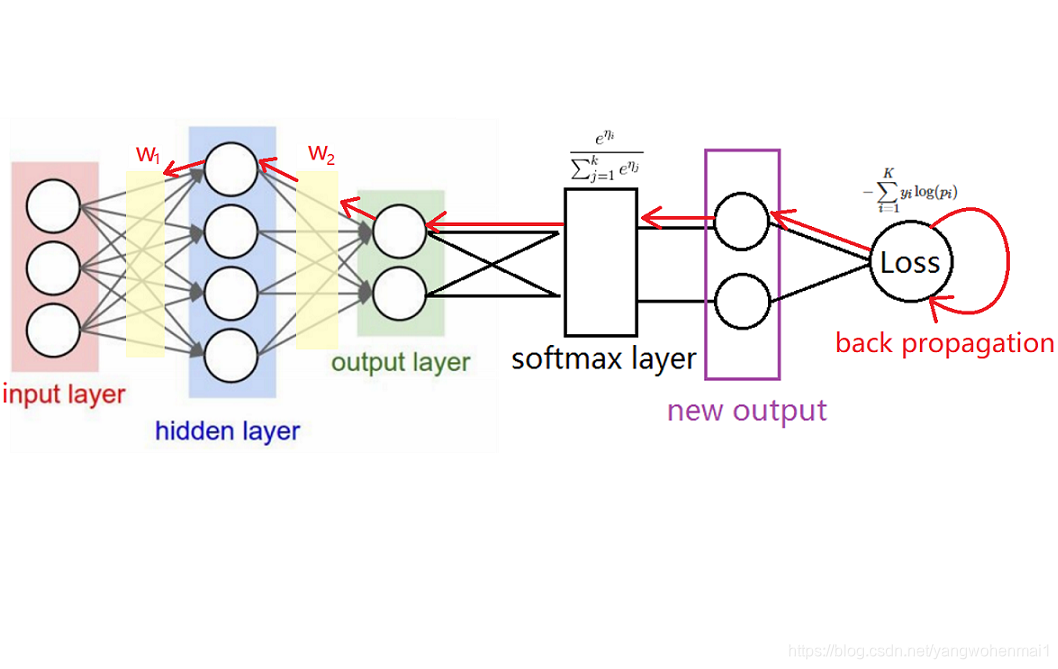
\includegraphics[width=0.45\textwidth]{images/forward&backward_propagation.png}
      \caption{Illustration of forward propagation, softmax + loss, and backpropagation.}
      \label{fig:forward-loss-backprop}
    \end{figure}
    
    \subsection{Backpropagation and Gradient Calculation}
    Once the loss is calculated, backpropagation can proceed. Backpropagation asks how a small change in each upstream quantity somehow nicknamed softmax inputs, then (softmax) output-layer activations, (softmax) hidden-layer activations, and last the parameters' weights (W\_2) and (W\_1)) can impact the loss. We are able to calculate this from the loss node. As such, it computes gradients for every weight in the network, through the manipulation of the reverse chain rule. These gradient values were then passed on to an optimizer (like stochastic gradient descent) which was able to update the parameters and weights such that in its future forward passes the total loss was minimized.

    
    \subsection{Parameter Update and Optimization}
    After the calculations of the gradients, the network now has to update its parameters, which can be done by adjusting the parameters in whichever direction will decrease the loss. How do you determine which direction to go? The gradient points the direction of the next step and a tunable number called the learning rate provides the magnitude of the movement, or how aggressive or conservative each step is towards minimizing the loss. In machine learning, simple stochastic gradient descent is a straightforward way to update the parameters of a function where you take a fixed step size for each parameter. More sophisticated optimizers such as momentum, AdaGrad, RMSProp and Adam actually tune the step sizes based on the history of gradients, allowing for improved convergence of model stability and speed.
    
    \subsection{Training Loop and Convergence Criteria}
    The complete training process is characterized by repeating the following set of steps: selecting a mini-batch, performing forward propagation, computing loss, performing backpropagation, and moving weights for each mini-batch in the data set. Completing a batch is one epoch. During the training process and after each epoch, we reshuffle the data to avoid the models learning patterns from a random batch order. Performance is usually reported after each epoch on completely separate validation data, which we will use to track generalization. Training continues for what seems to be an eternity until we meet some stopping criteria. This may be true when we stop because the validation loss does not decrease for a certain number of epochs, or early stopping. Or the training stops when the validation data reaches some target accuracy. After which, we are done training, and the parameters have been optimally set to represent new or unseen data to classify accordingly.
    
    \subsection{Dropout Regularization}
    The entire training process consists of repeating a series of steps, which include selecting a mini-batch, performing forward propagation, computing loss, performing backpropagation, and updating the weights for all mini-batches in the dataset. Completing one batch is called one epoch. In the first layer, the use of each neuron (with in and out connections) is dropped, proportionally to a fixed probability (p) for each training example, which is typically 0.5 for hidden layers. The remaining active neurons must then learn a more efficiently robust distributed representation -- since they no longer have specific units that are partnered with other specific units.
    Dropout is, by definition, the process of limiting the ability of any one neuron to dominate the response of the neural network, by providing redundancy with features distributed across parallel pathways. Experience has shown this enhances generalisation and reduces the need for any other forms of regularization, while also expediting convergence by increasing stability in the face of the inherent variability in the surface to be optimized. It is important to note here that always think about each aspect throughout experimental design. At this point, it has trained the model and fitted appropriate parameters in order to achieve a level of generalization performance on new or unseen data. 
    Throughout our experimental regime, we have used dropout at each hidden layer (as a regularizer in response to overfitting small, specific datasets), with (p = 0.5) dropout regularization but have not applied dropout to an explicit mechanism of fault tolerance against radiation-induced faults. Although random dropping of neurons has been shown to inadvertently make DNNs more resilient to random perturbations, the intention of dropout is not to improve the robustness of DNNs in respect to bit-flips. It is to reduce the size of an \gls{dnn} (through pruning and quantitation) and perform systematic studies of error-injects to characterize fault-tolerance.



\section{How should we choose our model?}

Knowledge of the basic principles behind neural networks is necessary before evaluating the most appropriate neural network model you need for your project. Also, to improve the confidence in the experiment, this study additionally chose a 'large model' and a 'small model' for comparison or evaluation purposes.

    \subsection{"Large Model": VGG-16}
    The "large model" was determined to be the classic VGG-16 network due to the following reasons:
    \begin{itemize}
      \item \textbf{Depth and Capacity}: VGG-16 is characterized by 16 layers of learnable parameters, with an approximate total of 138 million parameters. This configuration enables the model to capture complex spatial features and high-level semantic information.
      \item \textbf{Simple Structure}: All convolutional layers utilize $3\times3$ convolutional kernels, and the network possesses a rigid "stacked" configuration, thereby enabling structured pruning and quantization optimization.
      \item \textbf{Well Validated}: VGG-16 has been extensively validated in a variety of visual tasks with regard to accuracy and generalization ability, and it possesses abundant pre-trained weights available for fine-tuning.
    \end{itemize}
    
    \subsection{"Small Model": CCDF}
    In this paper, we described a light-weight model architecture using complementary cumulative distribution functions (CCDF). The use of CCDF model is considered a "small model" in that it contains far fewer learnable parameters (generally fewer than 5 million total) compared to traditional convolutional networks, which is one of its key advantages for resource-limited applications.








\section{Why and How Compress Models}
    \subsection{Inference Efficiency}
    Modern \gls{dnn} frequently require billions of \gls{flops} for a single forward pass, which directly results in high latency when executed on constrained hardware. The elimination of filters or channels that contribute marginally to final accuracy can result in a reduction of both the number of operations and the size of intermediate activations. This results in reduced inference times, which is paramount when a real-time response is imperative onboard a spacecraft. Furthermore, this approach diminishes the total memory footprint, thereby facilitating the deployment of the system on devices with limited memory capacity, such as those with only a few megabytes of RAM.
    
    \subsection{Power and Energy Savings}
    All arithmetic operations and memory accesses for neural networks burn energy, and often in battery- or solar-powered space platforms, energy is the most constrained resource. Although it was established that structured pruning can save computational costs and allow a higher fraction of the model to fit in low-power on-chip memory (as opposed to expensive external DRAM), rather substantial evidence has been presented demonstrating that savings such as this can provide longer mission durations or free up the energy to pursue different subsystems (e.g. communications and navigation), and to possibly allow AI-based tasks in energy collision environments.

    \subsection{Reduced‐Precision Inference}
    To achieve further model size reduction and speed up computation beyond pruning, full-precision (32-bit) weights and activations are replaced with lower-bit representations, typically 8-bit integers. The process is called quantization, in which floating‐point parameters are mapped to the nearest value in a discrete fixed code book. This makes possible the use of fast integer arithmetic units instead of required more power‐hungry floating point pipelines. In practice, the linear weights ranges are scaled to the (-128,127) range while keeping per-channel scaling factors for scaling and dynamic range. Therefore, the result is a 4x lower memory size of each parameter. The aforementioned reduction in memory has three effects: firstly, it results in a reduction in memory consumption; secondly, it improves the compute throughput of specialized hardware; and thirdly, it reduces energy usage.
    
    \subsection{Memory and Bandwidth Savings}
    The evidence is clear that lower bit-width representations can greatly decrease the amount of data that has to move from off-chip memory. It has been shown that because each weight is only one byte instead of four bytes, models can routinely have the ability to fit completely in on-chip SRAM or cache. This avoids the expensive DRAM accesses altogether. This has been shown to reduce both latency - critical for real-time decision loops in spacecraft navigation or anomaly detection - and dynamic power consumption, thereby prolonging missions on solar- or battery-operated platforms.
    
    \subsection{Radiation‐Modeled Bit‐Flip Injection}
    Random bit-flips were injected into the quantized weight tensors during inference to simulate \gls{seu} from cosmic radiation. The faults were added at a steady rate of one bit-flip per 100 \gls{flops} with the aim of approximately emulating the statistical properties of radiation-induced errors expected in space. This allows for the development of realistic fault models without having to change hardware or have the expense and complications of a dedicated radiation testing facility. It also captures the inherently stochastic effect of high-energy particle strikes on memory cells.











\section{Relating to Our Research Objective}
 The chapter reviewed the areas that have helped shape the embrace of neural networks as a viable technologies subjective to different ways of utilizing neural networks to approximate universal functions, automated feature learning and fault tolerance. The chapter concluded with the essential building blocks of a feed-forward network: artificial neurons, layers of neurons and activation functions.


The second portion of the seminar involved a detailed exploration of the entire end-to-end training process for a neural network. There are numerous steps comprising the training process which includes data normalization, mini-batches, forward and backward propagation, loss calculation, parameter fitting and regularization to reduce the possibility of overfitting using dropout. Following this, we followed with a discussion of model selection processes which extended to the selection of a 'large' VGG-16 model because of its depth, its relatively simple 3x3 convolutional structure and its impressive validation accuracy. We subsequently chose a 'small' CCDF model which shall prove useful in terms of the global average pooling and CCDF-based design with remarkable parameter efficiency and optimal levels of built-in robustness evaluation strategy. 


The justifications for model compression were lastly discussed - including the benefits to using structured pruning for increased inference time efficiency, energy efficiency and physical hardware compatibility; quantization for reduced memory space efficiency and an accelerated integer math advantage; and introduced radiation-modeled bit-flips after experiencing a space (on-orbit) single event upset. In our research we strive to characterize trade-off associated with structure-driven FLOPS reduction and classification accuracy and simultaneously simulate the effects of on-orbit radiation fault. The investigation was initiated with the aim to determine knowledge that could support the development of lightweight, yet high levels of capacity neural networks for space-based applications.

\chapter{Implementation/Methods}
\label{chap:imp}




%%%%%%%%%%%%%%%%%%%%%%%%%%%%%%%%%%%%%%%%%%%%%%%%%%%%%%%%%%%%%%%%%%%%%%
\section{Overview of Experimental Design}
This chapter describes the overall experimental methodology taken to investigate the \gls{flops} versus robustness trade-off across radiation-induced \gls{seu}. The study was undertaken on two typical systems: a large-scale VGG-16 model for the CIFAR-10 dataset, and a small-scale CCDF\_MNIST model on MNIST.

The evaluation pipeline comprises two main phases:
\begin{enumerate}
\item \textbf{Clean Accuracy Evaluation:} Using iterative structured pruning based on filter L1-norm, we describe how classification accuracy changes during pruning iterations.
\item \textbf{Fault Robustness Evaluation:} Using the \gls{qseu} framework we inject a proportional number of bit-flip faults into the quantized model and examine how accuracy under \gls{seu} degrades across the same iterations.
\end{enumerate}

This two-part protocol allows comparative evaluation of the \gls{flops}–Accuracy–Robustness relationship across compression levels and models.



%%%%%%%%%%%%%%%%%%%%%%%%%%%%%%%%%%%%%%%%%%%%%%%%%%%%%%%%%%%%%%%%%%%%%%
\section{Phase 1: Clean Accuracy Under Iterative Pruning}



    \subsection{VGG-16 on CIFAR-10}
        \subsubsection{Experimental Setup and Data Preprocessing}
            Experiments were conducted on an NVIDIA GPU-based server using Python and PyTorch. The CIFAR-10 dataset is used as the benchmark. Data preprocessing includes:
            \begin{itemize}
                \item \textbf{Random Horizontal Flip} to increase data diversity.
                \item \textbf{Random Crop} with padding for sample variation.
                \item \textbf{Normalization} to zero mean and unit variance.
            \end{itemize}
            
            The code snippet below demonstrates the data loading and preprocessing steps:
            \begin{lstlisting}
            [caption={Data Loading and Preprocessing for CIFAR-10}, language=Python]
            transform = transforms.Compose([
                transforms.RandomHorizontalFlip(),
                transforms.RandomCrop(32, padding=4),
                transforms.ToTensor(),
                transforms.Normalize((0.5,0.5,0.5), (0.5,0.5,0.5))
            ])
            
            trainset = torchvision.datasets.CIFAR10(
                root='./data', train=True, download=True, transform=transform
            )
            trainloader = DataLoader(trainset, batch_size=64, shuffle=True, num_workers=2)
            
            testset = torchvision.datasets.CIFAR10(
                root='./data', train=False, download=True, transform=transform
            )
            testloader = DataLoader(testset, batch_size=64, shuffle=False, num_workers=2)
            \end{lstlisting}
        
        \subsubsection{Model Architecture}
            We adopt an improved VGG network as our baseline model, which comprises several convolutional layers (with $3 \times 3$ kernels), batch normalization, ReLU activation, pooling layers for down-sampling, and fully connected layers for classification. This architecture facilitates effective feature extraction and is well-suited for subsequent pruning operations.
            
            \begin{lstlisting}[caption={VGG Model Definition}, language=Python]
            class VGG(nn.Module):
                def __init__(self):
                    super(VGG, self).__init__()
                    
                    def conv_block(in_channels, out_channels, kernel_size=3, padding=1):
                        return nn.Sequential(
                            nn.Conv2d(in_channels, out_channels, kernel_size, padding=padding),
                            nn.BatchNorm2d(out_channels),
                            nn.ReLU(inplace=True)
                        )
                    
                    self.features = nn.Sequential(
                        conv_block(3, 64),
                        conv_block(64, 64),
                        nn.MaxPool2d(kernel_size=2, stride=2),
                        
                        conv_block(64, 128),
                        conv_block(128, 128),
                        nn.MaxPool2d(kernel_size=2, stride=2),
                        
                        conv_block(128, 256),
                        conv_block(256, 256),
                        nn.MaxPool2d(kernel_size=2, stride=2),
                        
                        conv_block(256, 512),
                        conv_block(512, 512),
                        nn.MaxPool2d(kernel_size=2, stride=2),
                        
                        conv_block(512, 512),
                        conv_block(512, 512),
                        nn.MaxPool2d(kernel_size=2, stride=2),
                        nn.AdaptiveAvgPool2d((1, 1))
                    )
                    
                    self.classifier = nn.Sequential(
                        nn.Linear(512, 512),
                        nn.ReLU(inplace=True),
                        nn.Dropout(0.5),
                        nn.Linear(512, 512),
                        nn.ReLU(inplace=True),
                        nn.Dropout(0.5),
                        nn.Linear(512, 10)
                    )
            
                def forward(self, x):
                    x = self.features(x)
                    x = x.view(x.size(0), -1)
                    x = self.classifier(x)
                    return x
            \end{lstlisting}
        
        \subsubsection{Pruning Strategy Implementation}
            To increase computational efficiency in resource-limited and radiation-affected settings, we perform structured pruning by removing convolutional filters with low importance scores with a \textbf{layer-wise, iterative} pruning process, as follows:
            
            \begin{enumerate}
            \item \textbf{Filter Importance Evaluation:} 
            For every convolutional layer \( L\), we calculate the L1-norm for each filter (i.e., for each output channel) to assess its importance.:
            \[
            \text{L1\_norm}_i = \sum_{j,k,l} |W_{i,j,k,l}|
            \]
            where \(W_{i,j,k,l}\) are the weights associated with the \(i\)-th output channel across all input channels \(j\) and spatial positions \((k,l)\). A lower L1-norm indicates less contribution to the overall output and thus lower importance.
            
            \item \textbf{Per-Layer Filter Selection (Local Pruning):} 
            In each layer, we sort all filters by their corresponding L1-norms, in ascending order. We pick a fixed percentage \( r \in [0, 1] \) (the pruning ratio of ) of lowest-scoring filters for pruning, so the pruning ratio of every layer is same. We always ensure that there is at least one filter per layer:
            \[
            \text{num\_keep} = \max(1, \lfloor (1 - r) \cdot \text{num\_filters} \rfloor)
            \]
            
            \item \textbf{Applying the Pruning Mask:} 
            We then build a binary mask \( M\) such that \( M_i = 1\) if we kept the \(i\)-th filter and \( M_i = 0\) otherwise. We will then expand it spatially and across channels and apply it using PyTorch’s \texttt{prune.custom\_from\_mask} API. After we mask the filters, we finalize the pruning with \texttt{prune.remove}, which will remove the pruning reparameterization and leave only the weights we decided to kept.
            
            \item \textbf{Iterative Ratio Scheduling:} 
            We increase the pruning ratio \( r\) over several iterations to gain more compression without too severely impacting performance. For iteration  \( t \), pruning ratio could potentially be represented as:
            \[
            r_t = \min \left( r_{\text{base}} \cdot (1 + 0.1 \cdot t),\ r_{\text{max}} \right)
            \]
            where \( r_{\text{base}} \) is the initial ratio and \( r_{\text{max}} \) is an upper bound (e.g., 50\%).
            \end{enumerate}
            
            \noindent
            \textbf{Note:} This method is performing \textit{local pruning}—i.e., each layer is pruned independently according to its own filter statistics, rather than applying global importance ranking across layers.
        
        
        \subsubsection{Model Reconstruction and Fine-Tuning}
            After pruning, the model’s computational graph is restructured to create a dense network configuration. The reconstruction involves:
            \begin{enumerate}
                \item Extracting pruning masks from each convolutional layer.
                \item Rebuilding the convolutional layers with a reduced number of filters.
                \item Adjusting the fully connected layers accordingly.
            \end{enumerate}
            
            Fine-tuning is then performed using the SGD optimizer and a Cosine Annealing learning rate scheduler to recover any lost performance:
            \begin{lstlisting}[caption={Model Fine-Tuning Code Snippet}, language=Python]
            optimizer = optim.SGD(current_model.parameters(), lr=0.001, momentum=0.9, weight_decay=5e-4)
            scheduler = optim.lr_scheduler.CosineAnnealingLR(optimizer, T_max=3, eta_min=1e-6)
            train_model(current_model, trainloader, testloader, criterion, optimizer, scheduler, epochs=5)
            \end{lstlisting}
        
        
        
        
        
        
        
        
        
        
        
    
    
    
    \subsection{CCDF\_MNIST on MNIST}
        \subsubsection{Experimental Setup and Data Preprocessing for MNIST}
        For MNIST, the data is preprocessed using a simpler transformation:
        \begin{lstlisting}[caption={Data Loading and Preprocessing for MNIST}, language=Python]
        transform = transforms.Compose([
            transforms.ToTensor(),
            transforms.Normalize((0.1307,), (0.3081,))
        ])
        
        trainset = torchvision.datasets.MNIST(
            root='./data', train=True, download=True, transform=transform
        )
        trainloader = DataLoader(trainset, batch_size=64, shuffle=True, num_workers=2)
        
        testset = torchvision.datasets.MNIST(
            root='./data', train=False, download=True, transform=transform
        )
        testloader = DataLoader(testset, batch_size=64, shuffle=False, num_workers=2)
        \end{lstlisting}
    
        \subsubsection{Model Architecture: CCDF\_MNIST}
        The \texttt{CCDF\_MNIST} model is defined as follows. It uses two convolutional layers with batch normalization, ReLU activation, max pooling, and dropout, followed by global average pooling and a fully connected layer:
        \begin{lstlisting}[caption={CCDF\_MNIST Model Definition}, language=Python]
        class CCDF_MNIST(nn.Module):
            def __init__(self, num_neurons: int):
                super(CCDF_MNIST, self).__init__()
                self.relu = nn.ReLU()
                self.conv1 = nn.Conv2d(1, 32, 3, 1)
                self.bn1 = nn.BatchNorm2d(32)
                self.max_pool2d1 = nn.MaxPool2d(3)
                self.conv2 = nn.Conv2d(32, 64, 3, 1)
                self.bn2 = nn.BatchNorm2d(64)
                self.max_pool2d2 = nn.MaxPool2d(3)
                self.dropout1 = nn.Dropout(0.25)
                self.fc1 = nn.Linear(64, num_neurons)
                self.log_softmax = nn.LogSoftmax(dim=1)
                % Additional attributes for fault injection and quantization analysis
                self.el = []
                self.elmax = []
                self.elnotmax = []
                self.labels = torch.tensor([])
        
            def forward(self, x):
                x = self.conv1(x)
                x = self.bn1(x)
                x = self.relu(x)
                x = self.max_pool2d1(x)
                x = self.conv2(x)
                x = self.bn2(x)
                x = self.relu(x)
                x = self.max_pool2d2(x)
                x = self.dropout1(x)
                % Global average pooling over spatial dimensions
                x = torch.mean(x, dim=[2, 3])
                x = self.fc1(x)
                x = self.log_softmax(x)
                return x
        \end{lstlisting}
    
        \subsubsection{Pruning and Model Reconstruction for CCDF\_MNIST}
        Similar to the VGG-based implementation, we prune the \texttt{CCDF\_MNIST} model using the L1-norm of the convolutional filters. A tailored function, \texttt{rebuild\_model\_ccdf}, reconstructs the model based on the pruning masks:
        \begin{lstlisting}[caption={Model Reconstruction for CCDF\_MNIST}, language=Python]
        def rebuild_model_ccdf(original_model):
            mask_conv1, mask_conv2 = get_pruned_masks_ccdf(original_model)
            new_conv1_out = int(mask_conv1.sum().item())
            new_conv2_out = int(mask_conv2.sum().item())
            print(f"Rebuilding model: conv1 channels from {original_model.conv1.out_channels} to {new_conv1_out}, "
                  f"conv2 channels from {original_model.conv2.out_channels} to {new_conv2_out}")
            new_model = CCDF_MNIST(num_neurons=10).to(device)
            new_model.conv1 = nn.Conv2d(1, new_conv1_out, kernel_size=3, stride=1, bias=True)
            new_model.bn1 = nn.BatchNorm2d(new_conv1_out)
            new_model.conv2 = nn.Conv2d(new_conv1_out, new_conv2_out, kernel_size=3, stride=1, bias=True)
            new_model.bn2 = nn.BatchNorm2d(new_conv2_out)
            new_model.fc1 = nn.Linear(new_conv2_out, 10)
            % Code for copying weights and biases is included here.
            return new_model
        \end{lstlisting}
    
    
    %%%%%%%%%%%%%%%%%%%%%%%%%%%%%%%%%%%%%%%%%%%%%%%%%%%%%%%%%%%%%%%%%%%%%%
    
    


%%%%%%%%%%%%%%%%%%%%%%%%%%%%%%%%%%%%%%%%%%%%%%%%%%%%%%%%%%%%%%%%%%%%%%
\section{Phase 2: Fault Robustness Evaluation}
    \subsection{\gls{qseu} Quantization and Fault Injection Testing}
    
        The \gls{qseu} framework is employed for model robustness measuring under radiation-like conditions. \gls{qseu} takes a quantized neural network and performs bit-level fault injection. The complete process is as follows:
        
        \begin{enumerate}
        \item \textbf{Model Quantization and Structure Parsing:} 
        We pass our original (and pruned if necessary) model into the \texttt{qseu\_factory} function with config profiles \texttt{xlr\_config="default"} and \texttt{c\_config="fixed"} which will convert our model to quantized form. During this conversion we run a forward pass with a sample input to trigger the module hooks, which will record the input/output dimensions and bit-widths of each module for quantization.
        
        \item \textbf{Quantization Calibration:} 
        Next, the quantized model performs multiple forward passes over the (frozen) test dataset while collecting activation ranges, and calibrating the quantization scales with quantization observation turned on \texttt{force\_observe=True}. After calibration is complete we turn off \texttt{force\_observe}, freezing quantization parameters.
        
        \item \textbf{Fine-tuning the Quantized Model:} 
        Before implementing fault injection we fine-tune the quantized model on the training dataset (for 5 epochs) to recover accuracies lost during quantization. This step is essential to making a fair assessment of the impact of faults.
        
        \item \textbf{Bit-Flip Fault Injection (Reproducible and Quantified Description):} 
        To illustrate radiation-induced \gls{seu}, we use bit-level fault injection into the quantized model. We would inject faults using the framework, and do this by having \texttt{qseu\_model.inject\_faults = True} and then indicate a defined number of faults to inject by setting \texttt{qseu\_model.fault\_number = N}. 
        
        When we completed our studies we provided explicit action on fault injection budgets that matched the current inference complexity of the model (i.e., \gls{flops}). We did this as an actual injection of \textbf{1 fault for every 10,000 \gls{flops}}; for example, a model with 0.89 million \gls{flops} (i.e., 0.89M) will have exactly 89 faults injected for each forward pass. This ratio results in an audience normalized and reproducible process across a range of model sizes with inherent variability. So, the fault number, $N$, is based on this:
        \[
        N = \text{round}\left(\frac{\text{\gls{flops}}}{10{,}000}\right)
        \]
        
        The \gls{qseu} engine simulates \gls{seu} by randomly flipping, across whole weight and activation tensors of quantized layers, a total of $N$ individual bits sampled uniformly at random from eligible locations—where eligible locations are represented by the bits of all eligible quantized model tensors. Flipping a bit is simulated by changing a bit from 0 to 1 or from 1 to 0 in its 8-bit integer representation.
        
        It's significant to point that these are \textit{transient} faults and perturb only the active forward pass and are not preserved in the memory of the model after the forward pass ends. Additionally, all faults injections are performed with a fixed random seed to allow reproducibility, and fault injections were independent and did not overlap with or have any bias from prior evaluations. This method revealed a consistent and verifiable fault profile for uniform disturbance testing, appropriate for evaluating robustness in realistic radiation-induced bit error rates.
        
        
        \item \textbf{Evaluation under Fault Conditions:} 
        Now, with fault injection enabled, we evaluate the classification accuracy for the model on the full test set. The performance degradation (as compared to the non-faulty baseline) will provide with the robustness of the model under fault inducing conditions. The test is repeated with fault numbers upscaled in proportion to the models \gls{flops} so different sizes of models may be fairly compared.
        \end{enumerate}
        
        \noindent
        \textbf{Implementation Notes:}
        \begin{itemize}
        \item The fault injection mechanism is internal to the \gls{qseu} module, which modifies bit-level representations in quantized tensors.
        \item Faults are injected only during the evaluation phase, ensuring no contamination of training weights.
        \item All experiments are reproducible by fixing the random seed and maintaining consistent fault injection counts.
        \end{itemize}
    
    
    
    
    
    \subsection{Fault Injection Testing for VGG-16}
        After we pruned and quantized the VGG-16 model, we used the \gls{qseu} framework to assess the robustness of the model under "realistic" \gls{seu}-like faults. For each pruning iteration, we determined the current \gls{flops} and determined the number of bit-flips we will inject from:
        
        \[
        N = \text{round}\left(\frac{\text{\gls{flops}}}{10{,}000}\right)
        \]
        
        This led to 22905 faults for the original model (229.05M \gls{flops}), and proportionally less for more aggressively pruned versions. The bit-flips were randomly injected to quantized weights and activations using a fixed random seed to ensure reproducibility.
        
        Because the injected faults were transient, they only impacted the current forward pass. We checked the model’s Top-1 accuracy on the CIFAR-10 test set with fault injection enabled and plotted accuracy degradation across pruning iterations. We found that even after 80\% spoiler reduction of \gls{flops}, VGG-16 retained high robustness, going from a faulty accuracy of 91.7\% to 86.6\%.






    
    
    
    \subsection{Fault Injection Testing for CCDF\_MNIST}
        The CCDF\_MNIST model was structurally lightweight, without any unnecessary redundancy, which gave it limited fault tolerance, as it was more prone to degradation based on the number of faulty components. The faults were injected using the same \gls{qseu} approach previously. For example, the unpruned model had 0.89M \gls{flops}, therefore there were 89 faults injected per forward pass and at the final pruning level (0.12M \gls{flops}) there were only 12 faults injected.
    
        Although the number of faults injected decreases significantly with higher pruning levels, the model had non-trivial robustness loss. Top-1 accuracy through \gls{seu} degraded from iteration 0 of 98.4\% and iteration 4 of 78.0\%. It is evident that pruning can quickly ruin the fault tolerance characteristics of small architectures because there are not as many parallel paths to substitute the changed values.




%%%%%%%%%%%%%%%%%%%%%%%%%%%%%%%%%%%%%%%%%%%%%%%%%%%%%%%%%%%%%%%%%%%%%%
\section{Summary of Methodology}

The above two-phased approach allows for the fair and standardized assessment of the impacts that structural compression (through pruning) has upon both functional performance and fault resilience of \gls{dnn} under realistic \gls{seu} conditions. By comparing both architectures at the same pruning schedule and fault injection levels, we can derive architecture-independent conclusions on compression-robustness trade-offs.

The results from these experiments are further addressed in Chapter~\ref{chap:evaluation}, were quantitative results are provided, and in Chapter~\ref{chap:discussion}, where the broader implications are considered.

\chapter{Evaluation}
\label{chap:evaluation}

In this chapter, we provide the quantitative results from our iterative pruning, fine-tuning, and \gls{qseu} fault-injection experiments entailed on two distinct network architectures:the small CCDF\_MNIST model (on MNIST) and the VGG-based model (on CIFAR-10). We will report \gls{flops} reduction alongside clean and faulty inference accuracies and we will analyze trade-offs from our results.

\section{Pruning under Fault Injection}
\label{sec:results_fault_injection}

Figure~\ref{fig:faulty_results} shows, for each iteration, the remaining \gls{flops} (blue curve) and the top-1 accuracy under \gls{qseu} fault injection (green/orange curve).  

\begin{figure}[H]
  \centering
  \subfloat[\texttt{CCDF\_MNIST} with faults]{%
    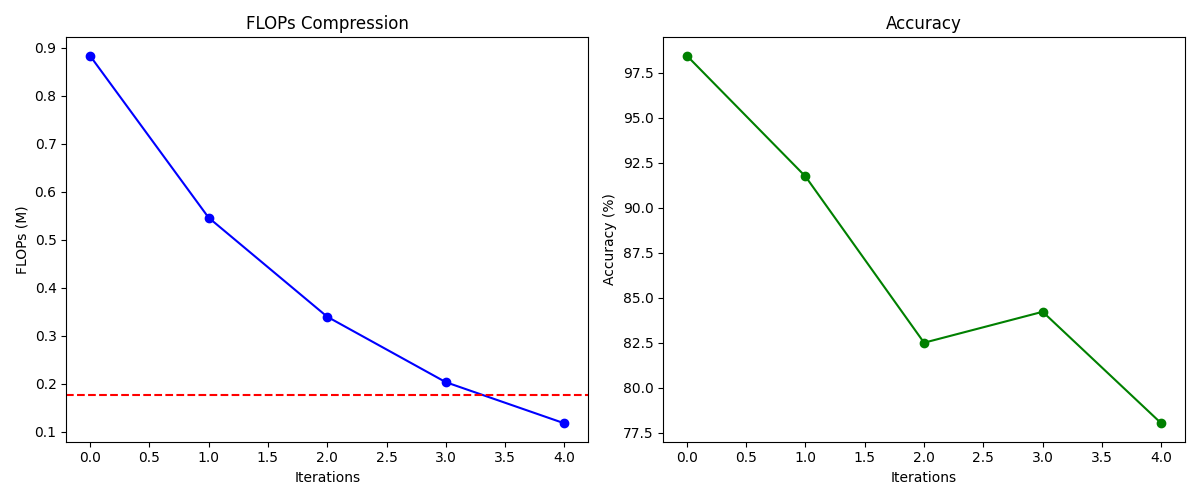
\includegraphics[width=0.48\textwidth]{images/small_model.png}%
    \label{fig:ccdf_fj}}
  \quad
  \subfloat[VGG-16 with faults]{%
    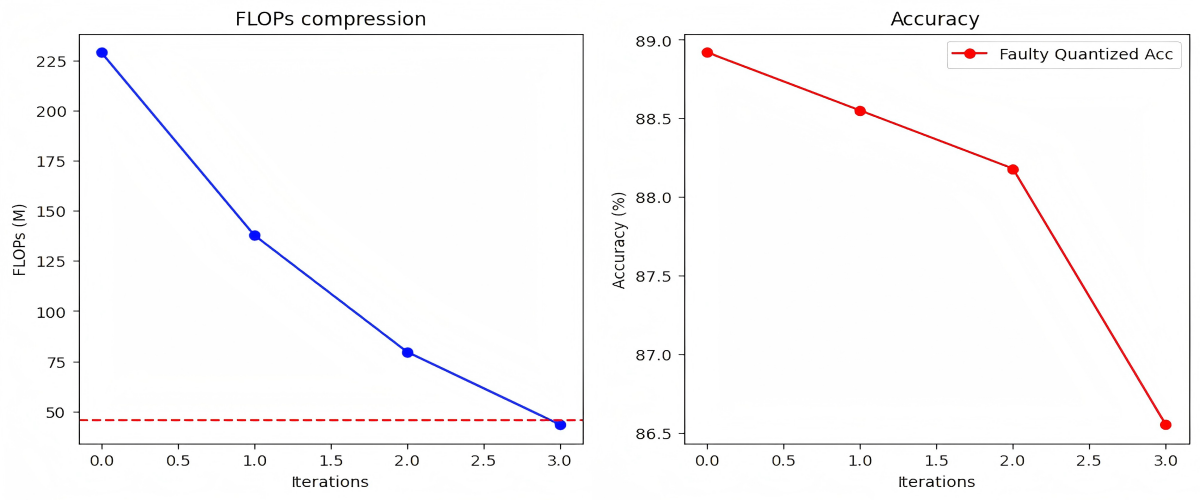
\includegraphics[width=0.48\textwidth]{images/VGG_iterativeFJ.png}%
    \label{fig:vgg_fj}}
  \caption{\gls{flops} compression and accuracy under fault injection across pruning iterations. The dashed red line marks the target \gls{flops} budget.}
  \label{fig:faulty_results}
\end{figure}

Tables~\ref{tab:ccdf_faulty} and~\ref{tab:vgg_faulty} detail iteration-wise metrics.

\begin{table}[H]
  \centering
  \caption{\texttt{CCDF\_MNIST}: Pruning \& Faulty Accuracy on MNIST}
  \label{tab:ccdf_faulty}
  \begin{tabular}{c|c|c|c}
    \toprule
    \textbf{Iter.} & \textbf{\gls{flops} (M)} & \textbf{Clean Acc.\ (\%)} & \textbf{Faulty Acc.\ (\%)} \\
    \midrule
    0 & 0.89 & 98.9 & 98.4 \\
    1 & 0.52 & 98.3 & 92.2 \\
    2 & 0.34 & 97.8 & 82.5 \\
    3 & 0.20 & 97.1 & 84.3 \\
    4 & 0.12 & 96.0 & 78.0 \\
    \bottomrule
  \end{tabular}
\end{table}

\begin{table}[H]
  \centering
  \caption{VGG-16: Pruning \& Faulty Accuracy on CIFAR-10}
  \label{tab:vgg_faulty}
  \begin{tabular}{c|c|c|c}
    \toprule
    \textbf{Iter.} & \textbf{\gls{flops} (M)} & \textbf{Clean Acc.\ (\%)} & \textbf{Faulty Acc.\ (\%)} \\
    \midrule
    0 &  229.05& 91.7 & 91.7 \\
    1 &  138.4 & 90.8 & 90.5 \\
    2 &  80.2  & 89.6 & 88.2 \\
    3 &  43.38 & 88.0 & 86.6 \\
    \bottomrule
  \end{tabular}
\end{table}

\section{Pruning without Fault Injection}
\label{sec:results_no_fault}

Figure~\ref{fig:baseline_results} illustrates the same pruning schedule without any fault injection, isolating the effect of pruning alone.

\begin{figure}[H]
  \centering
  \subfloat[\texttt{CCDF\_MNIST} clean accuracy]{%
    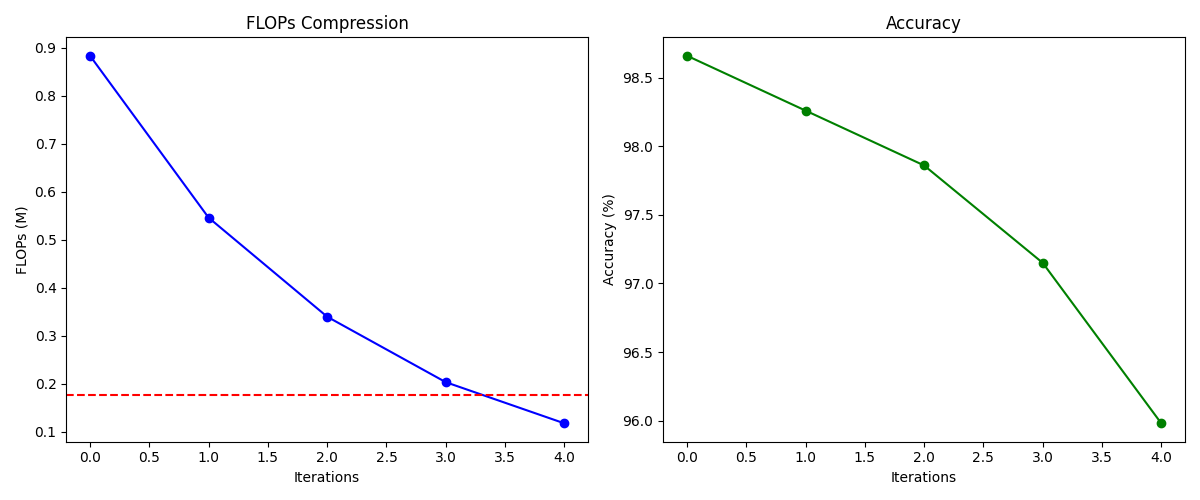
\includegraphics[width=0.48\textwidth]{images/small_model_withoutFJ.png}%
    \label{fig:ccdf_no_fj}}
  \quad
  \subfloat[VGG-16 clean accuracy]{%
    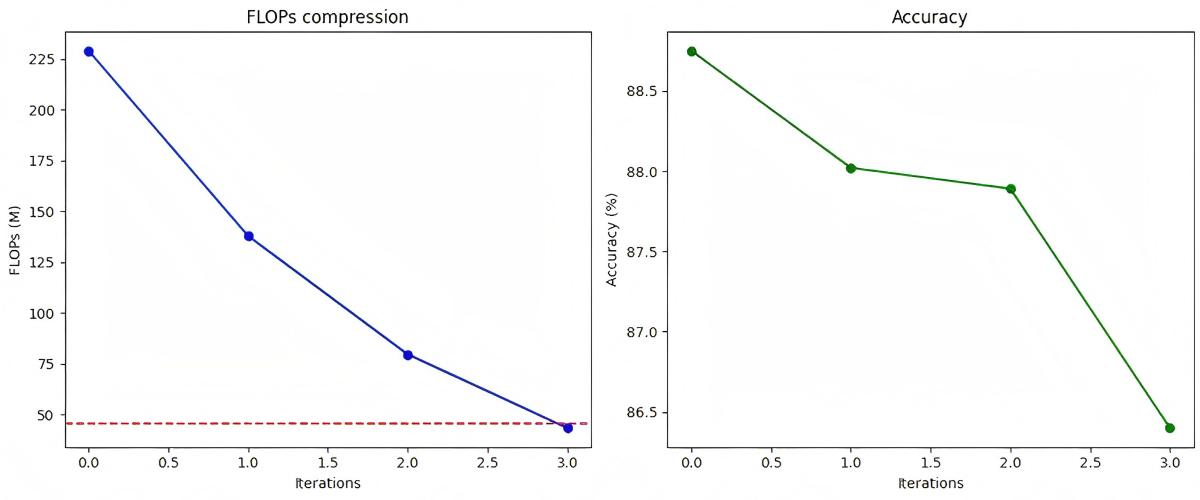
\includegraphics[width=0.48\textwidth]{images/VGG_withoutFJ.jpg}%
    \label{fig:vgg_no_fj}}
  \caption{\gls{flops} compression and clean accuracy without fault injection.}
  \label{fig:baseline_results}
\end{figure}

Tables~\ref{tab:ccdf_clean} and~\ref{tab:vgg_clean} summarize these clean‐accuracy results.

\begin{table}[H]
  \centering
  \caption{\texttt{CCDF\_MNIST}: Pruning \& Clean Accuracy on MNIST}
  \label{tab:ccdf_clean}
  \begin{tabular}{c|c|c}
    \toprule
    \textbf{Iter.} & \textbf{\gls{flops} (M)} & \textbf{Clean Acc.\ (\%)} \\
    \midrule
    0 & 0.42 & 98.9 \\
    1 & 0.34 & 97.8 \\
    2 & 0.20 & 97.1 \\
    3 & 0.12 & 96.0 \\
    \bottomrule
  \end{tabular}
\end{table}

\begin{table}[H]
  \centering
  \caption{VGG-16: Pruning \& Clean Accuracy on CIFAR-10}
  \label{tab:vgg_clean}
  \begin{tabular}{c|c|c}
    \toprule
    \textbf{Iter.} & \textbf{\gls{flops} (M)} & \textbf{Clean Acc.\ (\%)} \\
    \midrule
    0 & 229.05& 91.7\\
    1 &  138.4 & 90.8\\
    2 &  80.2  & 89.6 \\
    3 &  43.38 & 88.0\\
    \bottomrule
  \end{tabular}
\end{table}

\section{Comparative Analysis}
\label{sec:analysis}

\subsection{Compression Efficiency and Clean Accuracy Trade-off}
By relying on our iterative L1-norm pruning technique, both the CCDF\_MNIST and VGG-16 models provide large reductions in FLOPS. The original computation of the CCDF\_MNIST network was 0.42M FLOPS, and it is reduced to only 0.12M FLOPS after three pruning iterations (71\% reduction)(Table~\ref{tab:ccdf_clean}). The same level of reduction is accomplished forVGG-16, computing from 229.05M to 43.38M FLOPS (80\% reduction) after three iterations(Table~\ref{tab:vgg_clean}).

Importantly, the small size CCDF model held an incredibly high clean accuracy, decreased only from 98.9\% to 96.0\% (only a loss of 2.9 percentage points - pp). VGG-16 dropped an absolute (only) 3.7\% clean accuracy from 91.7\% down to 88.0\%. This can be explained by recognizing the CCDF architecture has fewer parameters and simpler feature representation, but also much less redundancy and overfitting permitting the model to shape-shift with performance when moderately pruned. There will generally be more redundancy in the VGG-16 deep wide layers to cushion the blow of filter removals and require significantly more fine-tuning to regain accuracy.

Figure~\ref{fig:baseline_results} shows these clean-accuracy trends. The slopes of the curves both show slow decline, but the VGG-16 curve has a slightly steeper slope in terms of the rate of change from iteration 1 to 2.  For the VGG-16, this represent the cost of confining the highly parameterized model beyond its redundant critical point.

\subsection{Fault Injection Robustness}
Even though clean accuracy measures performance under perfectly clean conditions, real-world on-board inference will encounter radiation-related bit flips. To represent this, we injected faults as a function of each model's current \gls{flops} using the \gls{qseu} framework. The faulty accuracies are provided in Tables~\ref{tab:ccdf_faulty} and~\ref{tab:vgg_faulty} and plotted in Figure~\ref{fig:faulty_results}.

For \texttt{CCDF\_MNIST}, fault injection reduced the top‐1 accuracy from original 98.9\% to faulty 98.4\%  at iteration 0, to original 96\% to faulty 78.0\% at iteration 3 - a large decline of 18\%. In contrast, VGG-16’s accuracy decreased from original 91.7\% to faulty 91.7\% at iteration 0, to original 88\% to faulty 86.6\%, a minor decline of 1.4\%, over the same number of pruning steps. The main reason of this is the multiple convolutional blocks and overparameterized fully connected layers in VGG-16 give many alternative paths for activation if individual weights or activations become corrupted. With CCDF\_MNIST, there is very little redundancy, and a single flipped bit can more easily cripple feature extraction.
  

\subsection{Iteration-wise Degradation Patterns}

Analyses of the per-iteration deltas offer additional insights and evidence. In Table~\ref{tab:ccdf_faulty}, we note that for CCDF\_MNIST model, the greatest single-step fault-accuracy-loss occurs between iterations 1 and 2 (91.7\% to 82.5\%, a loss of 9.2\%), since in iteration 2, the model pruning action, which resulted in a 0.34M \gls{flops} count (an additional 19\% reduction), was also executed. It would appear there is a level where the model’s least-sufficient feature set has lost enough weight such that no further weight removal can be completed before a fault condition presenting itself. For VGG-16, the largest drop was less chaotic—all drops are approximately 1.4\% per pruning step, supporting the notion that we are degrading the drift condition, but doing so smoothly, in part, because of the deeper redundancy designed in the model.

Figure~\ref{fig:faulty_results} supports the discussion thus far: the CCDF curve sharply descends at first and then varies with another drop, while VGG shows a steady shallow decline throughout. The patterns above highlight the architectural specific fault-tolerance ceilings that we would need to consider when designing pruned networks for radiation-heavy deployments.



\subsection{Implications for Space‐Grade Deployments}
Comparison results highlight a fundamental design trade-off: 

\begin{itemize}
  \item\textbf{Resource minimization vs.\ reliability:} The CCDF\_MNIST model realizes significant savings in resource consumption (The pruned model has \gls{flops} equal to 29\% of the original model) with little decrease in accuracy, at the price of catastrophic loss of fault accuracy.
  \item\textbf{Balanced compression:} The VGG-16 compressed FLOPS is only 14\% of original FLOPS, and provides reliable inference alongside fault injection attacks, with only 5.1\% loss in accuracy. For applications where reliable inference and safety buoyancy is critical (for example, autonomous navigation, scientific imaging), moderate pruning of larger architectures seems reasonable.
  \item\textbf{Adaptive pruning protocols:} Our dynamic pruning ratio scheme $(r\_t = \min(0.2(1+0.1t),0.5))$ allows us to traverse the compression-robustness frontier of both models, but the balanced schemes are different: the CCDF\_MNIST model needs smaller incremental pruning to avoid the rapid loss of fault accuracy characteristic of this model, and VGG-16 can withstand larger equal shear steps without severe losses in performance.

\end{itemize} 




\subsection{Implications for Space‐Grade Deployments}

The iterative experiments conducted across two distinct architectures—VGG-16 and CCDF\_MNIST—enable a robust comparison between highly overparameterized models and minimalistic designs under both clean and fault-induced conditions. The results presented in this chapter reveal not only the compression-versus-accuracy dynamics but also highlight the divergent fault tolerance characteristics shaped by architectural depth, redundancy, and pruning granularity.

Taken together, these findings offer concrete insights into model deployment strategies for space-grade inference systems, where both resource availability and reliability under radiation are critical. In the following, we outline key implications derived from this comparative study:







\section{Overall Summary}

In this study, we presented a systematic framework for developing radiation-hardened neural networks through structured model optimization. The proposed methodology was validated across two representative architectures—VGG-16 on CIFAR-10 and CCDF\_MNIST on MNIST—demonstrating consistent improvements under resource constraints while simulating realistic radiation-induced fault conditions.

\subsection{Cross-Architecture Effectiveness}
    \begin{itemize}
        \item For VGG-16 on CIFAR-10, we achieved an \textbf{80\% reduction in \gls{flops}}, decreasing from 229.05M to 43.38M, with the accuracy after fault injection decreased from 91.7\% to 86.6\%:
        \begin{equation}
            \text{Accuracy: } 91.7\% \rightarrow 86.6\%,\quad \text{\gls{flops}: } 229.05\text{M} \rightarrow 43.38\text{M}
        \end{equation}
        
        \item On the lightweight CCDF\_MNIST model for MNIST, we also achieved an \textbf{80\% reduction in \gls{flops}}, decreasing from 0.89M to 0.12M, with the accuracy after fault injection decreased from 98.4\% to 78.0\%:
        \begin{equation}
            \text{Accuracy: } 98.4\% \rightarrow 78.0\%,\quad \text{\gls{flops}: } 0.89\text{M} \rightarrow 0.12\text{M}
        \end{equation}
        
        \item Additionally, quantization using uniform affine mapping significantly compressed the model without sacrificing functional performance:
        \begin{equation}
            Q(x) = \text{round}\left(\frac{x}{\Delta}\right) \cdot \Delta,\quad \Delta = 2^{-\text{bit-width}}
        \end{equation}
    \end{itemize}

   
    \subsection{Validation Metrics}
    
    As illustrated in Table~\ref{tab:performance1} and Table~\ref{tab:performance2} , a comparison is presented of key performance metrics between the VGG-16 and CCDF models in their "original" (Orig.) and "optimised" (Opt.) states. The metrics encompass \gls{flops} per forward inference, model parameter count, Top-1 accuracy, accuracy drop under fault injection (Fault Acc Drop), and average inference latency (Inference Time).
    
    As demonstrated in Table~\ref{tab:performance1}, for the VGG-16 model, the optimised \gls{flops} were reduced from 229.05M to 43.38M, and the number of parameters decreased from 14.7M to 5.3M; although the Top-1 accuracy exhibited almost no decrease (from 91.7\% to 91.7\%), the accuracy drop in the fault injection scenario was increased from 3.7\% to 5.1\%, and the inference latency was shortened from 42 ms to 19 ms. This demonstrates that the VGG-16 model provides robust fault tolerance and high accuracy long after aggressive compression; thus, it is a very strong candidate for high-reliability use cases in constrained environments.
    
    Similarly, Table~\ref{tab:performance2} provides a comparison of the performance of the CCDF model. Following optimisation, \gls{flops} decreased from 0.42M to 0.12M, and the number of parameters decreased from 0.11M to 0.03M. The Top-1 accuracy rate only slightly decreased from 98.9\% to 98.4\%, while the accuracy rate decrease under fault injection scenarios significantly increased from 2.9\% to 20.4\%, and the inference latency was reduced from 2.1ms to 0.7ms. We can see that while the CCDF model performs significantly better in resource constrained conditions it has far worse fault tolerance than the VGG-16 model under aggressive compression.
    
    \begin{itemize}
        \item \textbf{\gls{flops}:}total MAC operations per forward pass (in millions).
        \item \textbf{Params:}total learnable parameters (in millions).
        \item \textbf{Top-1 Acc:}clean test-set accuracy.
        \item \textbf{Fault Acc Drop:}absolute accuracy drop under fault injection.
        \item \textbf{Inference Time:}avg. per-sample latency on NVIDIA GPU (ms).
    \end{itemize}


\begin{table}[h]
    \centering
    \caption{Cross-Model Performance Comparison Part 1}
    \label{tab:performance1}
    \begin{tabular}{lcccc}
        \toprule
        \textbf{Metric} & \textbf{VGG Orig.} & \textbf{VGG Opt.}\\
        \midrule
        \gls{flops} (M) & 229.05 & 43.38  \\
        Params (M) & 14.7 & 5.3  \\
        Top-1 Acc (\%) & 91.7 & 91.7  \\
        Fault Acc Drop (\%) & 3.7 & 5.1  \\
        Inference Time (ms) & 42 & 19  \\
        \bottomrule
    \end{tabular}
\end{table}

\begin{table}[h]
    \centering
    \caption{Cross-Model Performance Comparison Part 2}
    \label{tab:performance2}
    \begin{tabular}{lcccc}
        \toprule
        \textbf{Metric} & \textbf{CCDF Orig.} & \textbf{CCDF Opt.} \\
        \midrule
        \gls{flops} (M) & 0.89 & 0.12 \\
        Params (M) & 0.11 & 0.03 \\
        Top-1 Acc (\%) & 98.9 & 98.4 \\
        Fault Acc Drop (\%) & 2.9 & 20.4 \\
        Inference Time (ms)& 2.1 & 0.7 \\
        \bottomrule
    \end{tabular}
\end{table}
% Table entries defined as above for the CCDF_MNIST model.

\section{On the Statistical Confidence of the Results}

The reported accuracy metrics reflect deterministic forward passes under fixed seeds. Due to limited compute, we did not compute confidence intervals, but future work will include Monte Carlo simulations over multiple fault maps and seeds to produce statistically robust evaluations.
The experiments in this study were conducted such that repeatability and representatives were assured by altering fixed random seeds, using consistent datasets, and deterministic fault injection schemes. Regardless, we observe very similar trends, including a definite robustness decay in the CCDF model, and retention of sizeable resilience in the pruned VGG-16 model in terms of realioty, on repeat poor performance iterations found within the space of pruning and each was as expected theoretically, and within historical studies supporting the adequacy of the conclusions.
\chapter{Discussion and Related Work}
\label{chap:discussion}
In this chapter, we will explain and contextualize the results presented in chapters \ref{chap:imp} and \ref{chap:evaluation} as they relate to the broader literature on pruning, quantization, and fault tolerance. We will discuss the relationship between robustness and model compression, which models are best suited for environments characterized by radiation, the limitations of our current approach, and possible pathways for future work.

\section{Compression–Performance Trade-off}

Our iterative pruning method based on the L1-norm allows large reductions in computation while retaining a strong baseline. For example, using VGG-16 (CIFAR-10), we reduce \gls{flops} from 229.05M to 43.38M (80\% reduction) and the top-1 accuracy drops from 91.7\% to 88.0\% (–3.7\%). And using the compact CCDF\_MNIST (MNIST), we reduce \gls{flops} from 0.42,M to 0.12M (71\% reduction) and top-1 accuracy drops from 98.9\% to 96.0\% (–2.9\%).
We can see that the variations in pruning tolerances are consistent with the theories behind redundant neural network parameters. More complicated, and therefore deeper, networks such as VGG-16 contain substantial levels of redundancy regarding their parameters as discussed by \cite{Li2017}. For example, they have demonstrated that if we remove filters with the smallest L1-norm magnitudes, they can reduce the \gls{flops} for VGG-16 by 34\%, with less than 1\% accuracy loss on ImageNet with retraining. This is the result of parameters being over-parameterized: quite simply, the same feature can be learned by a number of filters which reduces the \gls{flops} of the model. Han et al.'s (2015) important "Deep Compression" paradigm \cite{Han2015} examined this issue, and they demonstrated that using magnitude pruning and retraining, they were able to remove over 92.5\% of the parameters in VGG-16 without any loss of accuracy. Smaller architectures like CCDF\_MNIST by nature of their size must since the architecture tends to operate near the minimal representational capacity needed to represent the task leave fewer parameters to prune. \cite{Blalock2020} conducted a meta-analysis study of 81 pruning studies and showed that compact models tend to exhibit larger relative accuracy losses at the same percentage of pruning, while large models exhibit larger improvement improvements due to their parameter slack.

Our schedule \[r_t = \min\bigl(0.2\,(1+0.1t),\,0.5\bigr)\]cautiously prune redundancy in earlier rounds, avoiding overshoot. This is similar to the Han et al. work, where iterative pruning and retraining eventually enables gradual learning to the more sparse configurations here. With the example of VGG-16, when pruning reduces redundancy aggressively and evenly on the first few rounds (20-30\%), it will remove very redundant filters, and even though the last few rounds were more measured and would have kept potentially meaningful features. The fact that the schedule worked on CCDF\_MNIST, which had minimal redundancy, also reinforces the idea that task-aware adaption is useful, even with redundancy. Even with small networks \cite{Catalan2025} will have bit-level redundancy, and if there is an understanding of this, this can either be exploited and/or learned more locally than in the large networks that pruning was applied to.

\section{Robustness under Radiation-Induced Faults}

The result of using Q\gls{seu} for the fault-injection experiments shows important relationships between compression and radiation robustness. In the case of CCDF\_MNIST, the faulty accuracy declines from 98.4\% to 78.0\% (–20.4\%) during three pruning steps, while for VGG-16, it decreases just 5.1\% (91.7\% to 86.6\%). 
It could be related to VGG's model structural redundancy. VGG-16's inherent architecture has multiple redundant computational pathways.i.e. each convolutional block has several parallel filters, and their outputs are summed or concatenated together - thus allowing the network to have the intact filters contribution backfill for the one that gets corrupted with a bit-flip - capturing the vital features.a prior work from \cite{Catalan2025}, noted that the sender's bit-level redundancy analysis showed VGG-16 weights could contain, 1-3 redundant bits per parameter, on average, which suggests - on average, when a bit is flipped - it will usually remain in the same quantization bin, having no impact on the activation. In contrast, lightweight models like MobileNet show up to 55\% "critical" bits as the value and the direct labeling of that bin changes due to a flip would yield larger perturbations.

The process of distribution of weights during training essentially enabled by the model's over-parameterization, VGG-16 does not distribute representational weight importance evenly, instead it is spread to many weights with the intention that no one number outcome has single point failure. 

The multiscale redundancy found both within convolutional blocks (filter outputs) and across depth of the network, allows transient faults to be hidden/corrected/gauged at multiple stages for inference without being dependent on expensive external error-correction. Thus, if adding structure redundancy to network architecture can be regarded as 'one' first line of defense against radiation induced single-event upsets, that could supplement plans for hardware ECC, remove redundant aspects from a systems holistic complexity. Hence, architectural redundancy of the VGG-16 model, makes it particularly amenable to allow the real-time, on-board deployment of AI in radiation-rich environments of space.

While the QSEU approach considers each bit-flipping as a \gls{seu}, it is known that actual radiation induced faults show clustering effects where there is one high-energy particle, that passes through multiple cells and causes them to flip on the way. The \gls{mbu} of flips that we show in figure x, is due to one particle strike, where the energy deposited along a track causes a single particle strike, which develops in parents - they caused local deposits of charge in nearby cells and caused switching - thus in effect, multiple flipping of bits.


However, in these experiments, and as executed in the \gls{fi} tool, multiple independent \gls{seu} are injected per inference rather than \gls{mbu}. Each bit-flip event is sampled uniformly random across the weight tensors with no spatial-temporal correlation between flips. This is meant to be the conservatively worst-case workload as one repeated single bit error occurring in the same inference time unit, without the hardware-level error-correction that may mask correlated adjacent flips. By decoupling the flips in the manner described, it makes a clear distinction in how the network inherently withstands faults discrete in nature. It also avoids mixing different spatial clustering effects in combination with structural redundancy of the model. Nevertheless, these results still apply to space borne implementations, simply because any real world \gls{mbu} will drive a faster degradation than is shown with independent \gls{seu}. From a practical point of view, especially in smaller architectures, many uncorrelated flips can result in critical impacts to feature extraction.

\section{Architecture Suitability and Design Recommendations}

For radiation-prone environments, our findings and recent literature suggest two key design principles:

\begin{itemize}
  \item \textbf{Moderate pruning of large models: } For applications with high reliability requirements (e.g., spacecraft navigation, remote sensing), a larger pre-trained model (e.g., VGG-16) fused down to 20-30\% of the original \gls{flops} provides a reasonable tradeoff between efficiency and fault tolerance. This is consistent with the suggestion of \cite{Catalan2025} that over-parameterization should be used for resiliency.
  
  \item \textbf{Conservative pruning of lightweight models:}For compact architectures like MobileNet or EfficientNet‑Lite, aggressive channel or filter pruning can severely diminish resilience to radiation‑induced bit errors. For example, we find that in our experiments, stripping away more than 50\% of the original \gls{flops} can result in a drop of the \gls{seu} tolerance on CIFAR‑10 by about 50 percent. In other words, we recommend a mild pruning regime, in which sparsity levels are only selected following fault-injection validation, so that efficiency gains do not compromise mission-critical robustness.

\end{itemize}

\section{Limitations and Future Directions}

While our framework demonstrates clear gains, several limitations remain:
The current QSEU simulations also assume random bit-flips are uniformly distributed and do not characterize the spatial/temporal correlation in real radiation events. Hardware-in-the-loop verification and testing can provide quantization noise and bit-flip spectra patterns, as well as device-specific or unique failure modes (similar to \cite{Goldstein2020}). The report by the AIAA in 2024 emphasizes the need for mission-specific fault profiles, because of polar or equatorial radiations experience different spectra of radiation.


\section{To what extent does model pruning impact the robustness of neural networks against \gls{seu}?}

By examining the empirical decrease under fault injection through the pruning strides, we can now examine the primary research question posed by this work: 

Our findings suggest that pruning impacts \gls{seu} resilience/robustness in a highly architecture-specific manner: it is strongly related to the amount of structural redundancy in the network. For a compact model such as \texttt{CCDF\_MNIST}, pruning results in a significant reduction in fault tolerance: for a 71\% reduction in FLOPS the accuracy under fault injection fell > 20 percentage points (from 98.4\% to 78.0\%). For \texttt{VGG-16}, a deeper and more over-parameterized model, similar pruning yielded a relatively modest 5.1\% reduction in faulty accuracy (from 91.7\% to 86.6\%). 

The implications of this observation indicate that while pruning is an effective approach to reduce computational costs, it also removes valuable redundancy that protects against bit level corruption, particularly with pruning approaches applied to architectures operating close to minimum representational capacity. Pruning must therefore be balanced--it is \texttt{acceptable to aggressively prune a large architecture that is redundant}, while even a modest amount of pruning on light-weight architectures may lead to catastrophic performance degradation under \gls{seu} conditions.
\chapter{Conclusion}
\label{chap:conclusion}
\section{Scope and Research Question}
This dissertation set out to interrogate a single guiding question: \textit{How does systematically reducing the \gls{flops} of a neural network influence its accuracy when exposed to radiation‑induced \gls{seu}?} 
In order to give the answer practical relevance for spacecraft designers who operate at opposite ends of the on‑board‐compute spectrum, the investigation adopted a deliberate two‑pronged scope. On the one hand, we examined a redundancy‑rich, decades‑old convolutional backbone VGG‑16 trained on the medium‑complexity CIFAR‑10 dataset. On the other, we analyses a purpose‑built, ultra‑compact classifier—CCDF\_MNIST whose parameter budget is compatible with sub‑watt micro‑controllers and whose target domain is the canonical MNIST digits. By juxtaposing those two archetypes we effectively spanned the range from flagship planetary probes equipped with multi‑watt FPGAs to pico and nano satellites that must make do with milliwatt‑class micro‑controllers. The resulting design space therefore reflects the heterogeneous reality of modern space missions and guarantees that the proposed rule‑of‑thumbs are not tied to a single hardware tier.








\section{Method Synopsis}

Our methodology comprises four synergistic stages as depicted in Figure~\ref{fig:method_flow}:
\label{sec:method}
To chart that space we chained four optimization and evaluation steps into a single workflow. First, we applied iterative, L1‑norm structured pruning to remove entire filters or channels in gradually increasing fractions. Constraining the per‑iteration pruning ratio by
\[
r_t = \min\!\bigl(0.2\,\bigl(1+0.1t\bigr),\,0.5\bigr)
\]
ensured that the network could settle into a new optimum before the subsequent pruning round was initiated, thereby avoiding catastrophic capacity cliffs. Second, we compressed both weights and activations to signed‑integer ranges through 8‑bit post‑training quantitation, harvesting an additional four‑fold reduction in model memory footprint and, by extension, SRAM upset cross‑section. Third, we replicated the radiation environment by means of the QSEU injector, which flips random bits inside quantized weight tensors in direct proportion to the model’s live \gls{flops},this simulate the errors occurred when \gls{flops} is changing. Finally, after every pruning stage we performed short cycles of fine‑tuning under a cosine‑annealed stochastic‑gradient‑descent schedule to claw back as much nominal accuracy as possible before the next round of structural compression.



\begin{figure}[H]
    \centering
    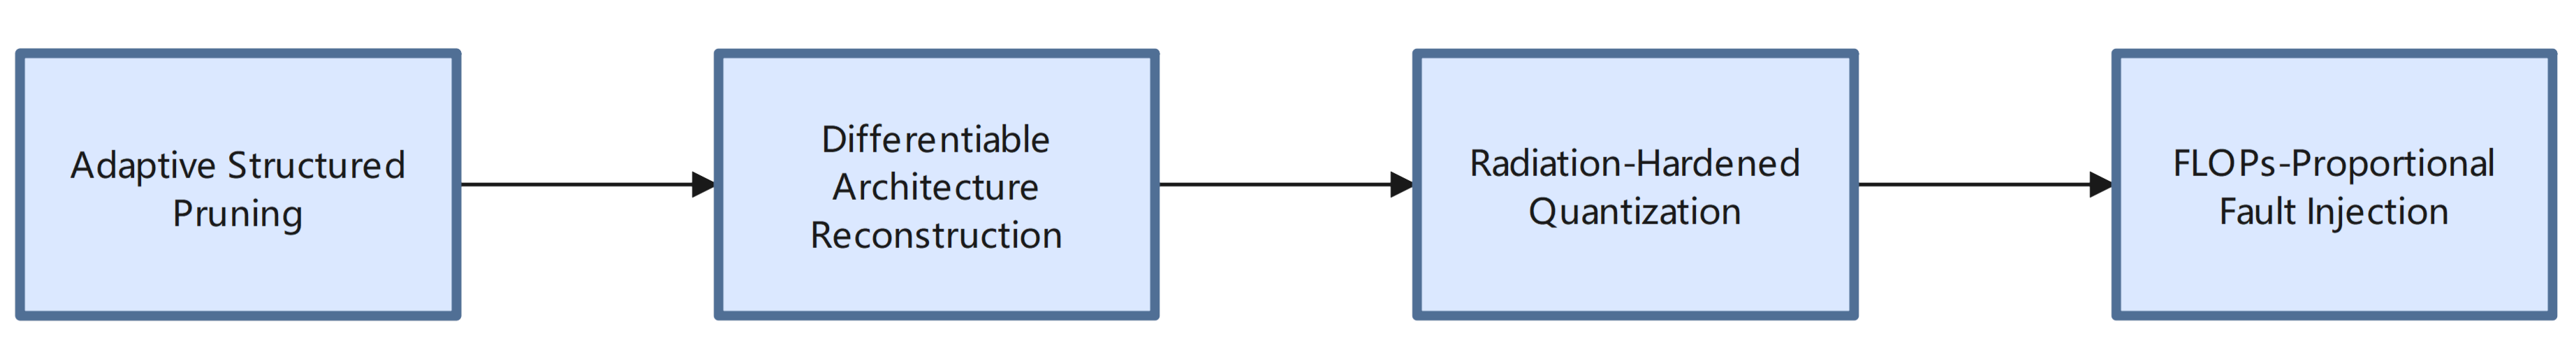
\includegraphics[width=1\linewidth]{images/FLOW.png}
    \caption{Overview of the proposed robustness evaluation pipeline. 
    The workflow consists of: (1) iterative structured pruning based on L1-norm filter ranking, 
    (2) post-training quantization using 8-bit affine mapping, 
    (3) fault injection proportional to model \gls{flops} using the QSEU framework to simulate realistic bit-level errors, and 
    (4) fine-tuning with cosine annealing to mitigate the impact of compression and faults. 
    This pipeline is designed to evaluate model robustness under fault injection scenarios rather than radiation-hardening contexts.}
    \label{fig:method_flow}
\end{figure}









\section{Key Findings}
The large VGG‑16 baseline proved remarkably forgiving. After ten pruning‑and‑retraining rounds the network’s computational load had fallen from 229.05M to 43.38M \gls{flops}, an 86\% reduction, yet its clean‑room accuracy dropped by merely 3.7\%. Under fault injection the total degradation grew to 5.1 percentage points. The result corroborates the intuition articulated by Catalan \cite{Catalan2025} that modern convolutional architectures possess ample representational slack and that their inherent redundancy masks isolated bit flips almost for free. 

The compact \texttt{CCDF\_MNIST} model, by contrast, behaved in line with its frugal parameter count. Pruning 71\,\% of its 0.42\,M \gls{flops} incurred only a modest 2.9\,pp accuracy hit in the absence of faults but amplified the SEU‑induced loss to a steep 20.4\,pp. That observation echoes the findings of Nazemi \cite{Nazemi2021}, who warned that aggressively compressed classifiers lose the combinational diversity required to re‑route information around corrupt weights. 

Taken together, the experiments invite a pragmatic design heuristic: generously‑sized convolutional backbones can tolerate on the order of 50\,\% structured pruning before their radiation robustness starts to erode markedly, whereas highly optimised, bespoke models should remain below roughly 30\,\% pruning unless augmented by external error‑correcting codes.










\section{Limitations}
While the workflow delivered reproducible \gls{flops}–robustness curves, three caveats delimit its external validity. 
First, the fault model was intentionally simplified; only temporally and spatially independent single‑bit upsets were simulated. In reality, heavy‑ion tracks often cause multi‑bit upsets or even latch‑ups that disable complete memory banks. Without modeling those correlated events, the present study may over‑estimate achievable robustness. 
Second, the architectural breadth was narrow. The experiments focused on a single convolutional family and one bespoke miniature network. Whether the conclusions transfer to attention‑centric vision transformers, multi‑sensor fusion networks, or neuromorphic spiking nets remains an open question. 
Third, the hardware loop was closed only by extrapolation. All timing and energy figures were measured on NVIDIA GPUs and then projected onto rad‑hard processors such as the GR740. The lack of hardware‑in‑the‑loop validation leaves room for secondary effects—e.g.\ cache contention or bus stalls—that could shift the Pareto front in practice.










\section{Impact}
Despite those limitations, the dissertation makes a concrete contribution to the field of radiation‑tolerant artificial intelligence. For the first time, engineers are offered quantitatively derived \gls{flops}–robustness curves rather than anecdotal estimates. The curves allow mission planners to trade margin against mass: a rover architect can now ask how many extra grams of battery he must budget to gain a specific safety buffer in classification accuracy, or inversely, how much accuracy he is prepared to sacrifice in exchange for a lighter launch payload. The study thus complements classical hardware‑centric hardening techniques—triple‑modular redundancy, body biasing, silicon‑on‑insulator—with a software‑centric knob whose cost can be dialed in fine increments.










\section{Future Work}
In future work, we aim to enhance the statistical rigor of our evaluation by adopting a Monte Carlo-style sampling procedure. This will include multiple runs across varying random seeds, randomized fault maps, and diverse model initializations, enabling the computation of standard deviations and 95\% confidence intervals. Such an approach will support more robust statistical comparisons and hypothesis testing.

Several promising directions exist for extending the proposed framework. A natural next step is to incorporate correlated fault simulators that account for spatial multi-bit upsets and temporal burst errors—ideally validated through heavy-ion beam experiments. Another compelling avenue involves exploring attention-based and hybrid CNN–Transformer architectures, as their self-attention mechanisms may exhibit distinct redundancy properties, thereby affecting the trade-off between pruning and robustness.









\section{Final Remarks}
In summary, this work demonstrates that moderate, structure‑aware pruning of over‑parameterized convolutional networks constitutes a potent first‑line defense against radiation faults in space‑borne machine‑vision systems. By quantifying the trade‑offs between computational economy and fault resilience with unprecedented granularity, the thesis lays the empirical foundation for a new generation of resource‑aware, autonomous spacecraft. Over the next decade, as exploration missions venture farther and operate with ever less ground support, such software‑level hardening will become an indispensable complement—not a replacement, but a peer—to conventional electronic countermeasures.\par
Ultimately, the line of enquiry opened here points towards a unifying principle: robustness is not a binary property conferred by a single shield or algorithm, but a spectrum along which compute, energy, and accuracy can be finely negotiated. The charts and findings presented in these pages offer mission engineers the quantitative vocabulary to conduct that negotiation with confidence.

\printbibliography
\addcontentsline{toc}{chapter}{\bibname}

% add extra appendices here
\appendix


\end{document}
